% ─────────────────────────────────────────────────────────────────────────────
% Психиатрическая геномика — Полный анализ (Русский)
% Евгений Щербинин · Bloomsbury Technology · Апрель 2026
% Компиляция: xelatex report_ru.tex
% ─────────────────────────────────────────────────────────────────────────────
\documentclass[11pt, a4paper]{article}

\usepackage[margin=2.4cm]{geometry}
\usepackage{fontspec}
\usepackage{polyglossia}
\setmainlanguage{russian}
\setotherlanguage{english}
\setmainfont{Palatino}
\newfontfamily\russianfont[Script=Cyrillic]{Palatino}
\setsansfont{Helvetica Neue}[Scale=0.92]
\setmonofont{Menlo}[Scale=0.88]

\usepackage{microtype}
\usepackage{graphicx}
\usepackage{booktabs}
\usepackage{array}
\usepackage{xcolor}
\usepackage{amsmath}
\usepackage{amssymb}
\usepackage{hyperref}
\usepackage{caption}
\usepackage{float}
\usepackage{enumitem}
\usepackage{titlesec}
\usepackage{fancyhdr}
\usepackage{parskip}
\usepackage{mdframed}
\usepackage{subcaption}

% ── Цвета ─────────────────────────────────────────────────────────────────────
\definecolor{accent}{HTML}{264653}
\definecolor{highlight}{HTML}{E63946}
\definecolor{muted}{HTML}{6c757d}
\definecolor{lightbg}{HTML}{f8f9fa}
\definecolor{sudcol}{HTML}{BC6C25}

% ── Типографика ───────────────────────────────────────────────────────────────
\titleformat{\section}{\large\bfseries\color{accent}}{}{0em}{}[\titlerule]
\titleformat{\subsection}{\normalsize\bfseries\color{accent!80!black}}{}{0em}{}
\titlespacing{\section}{0pt}{18pt}{6pt}
\titlespacing{\subsection}{0pt}{12pt}{4pt}

\hypersetup{colorlinks=true,linkcolor=accent,urlcolor=accent,citecolor=muted,
  pdftitle={Психиатрическая геномика — Полный анализ},
  pdfauthor={Евгений Щербинин}}

\captionsetup{font=small,labelfont=bf,skip=6pt}
\setlist[itemize]{leftmargin=1.5em,itemsep=2pt,parsep=0pt}

\pagestyle{fancy}\fancyhf{}
\fancyhead[L]{\small\color{muted}Психиатрическая геномика PGC · Полный анализ}
\fancyhead[R]{\small\color{muted}Bloomsbury Technology · \today}
\fancyfoot[C]{\small\color{muted}\thepage}
\renewcommand{\headrulewidth}{0.4pt}

\newmdenv[backgroundcolor=lightbg,linecolor=accent,linewidth=2pt,
  leftline=true,rightline=false,topline=false,bottomline=false,
  innerleftmargin=10pt,innerrightmargin=10pt,
  innertopmargin=6pt,innerbottommargin=6pt,
  skipabove=8pt,skipbelow=8pt]{callout}

% ─────────────────────────────────────────────────────────────────────────────
\begin{document}

% ── Заголовок ─────────────────────────────────────────────────────────────────
\begin{center}
  {\LARGE\bfseries\color{accent} Психиатрическая геномика в масштабе}\\[4pt]
  {\large Исследовательский анализ датасета OpenMed PGC GWAS}\\[3pt]
  {\normalsize\color{sudcol}\bfseries
    Включает: расстройства употребления психоактивных веществ —
    манхэттенский график, QQ-анализ и симуляция полигенного риска}\\[10pt]
  {\normalsize Евгений Щербинин \quad|\quad Bloomsbury Technology \quad|\quad \today}\\[2pt]
  {\small\color{muted}
    \href{https://huggingface.co/collections/OpenMed/pgc-psychiatric-gwas-summary-statistics}%
    {\texttt{OpenMed/pgc-psychiatric-gwas-summary-statistics}} · Hugging Face}
\end{center}
\vspace{4pt}\hrule\vspace{14pt}

% ── Аннотация ─────────────────────────────────────────────────────────────────
\begin{abstract}
\noindent
Организация OpenMed стандартизировала все мета-анализы полногеномных
ассоциативных исследований (GWAS), опубликованные Психиатрическим геномным
консорциумом (PGC), в единую коллекцию на Hugging Face:
\textbf{1,14 миллиарда строк}, \textbf{12 психиатрических нозологий},
\textbf{52 ключевых исследования}. В данном отчёте представлены:
профилирование схем данных, характеристики частот минорных аллелей,
кросс-нозологические корреляции генетических эффектов по 489~904 общим
SNP, а также расширенный анализ подисследования \textbf{SUD2023}
(расстройства употребления психоактивных веществ), включающий
манхэттенский график, QQ-диаграмму ($\lambda_\text{GC} = 1{,}492$,
13 геномно-значимых хитов в выборке), профиль кросс-нозологических
корреляций и симуляцию полигенного оценочного риска (PRS) в рамках
модели порога ответственности.
\end{abstract}
\vspace{8pt}

% ─────────────────────────────────────────────────────────────────────────────
\section{Обзор датасета}
% ─────────────────────────────────────────────────────────────────────────────

Каждая строка представляет собой тест ассоциации SNP--фенотип: идентификатор
варианта, хромосома, позиция, аллели, размер эффекта (BETA или OR), стандартная
ошибка, p-значение, качество импутации, частота аллелей и объём выборки
(N, Nca, Nco).

\begin{figure}[H]
  \centering
  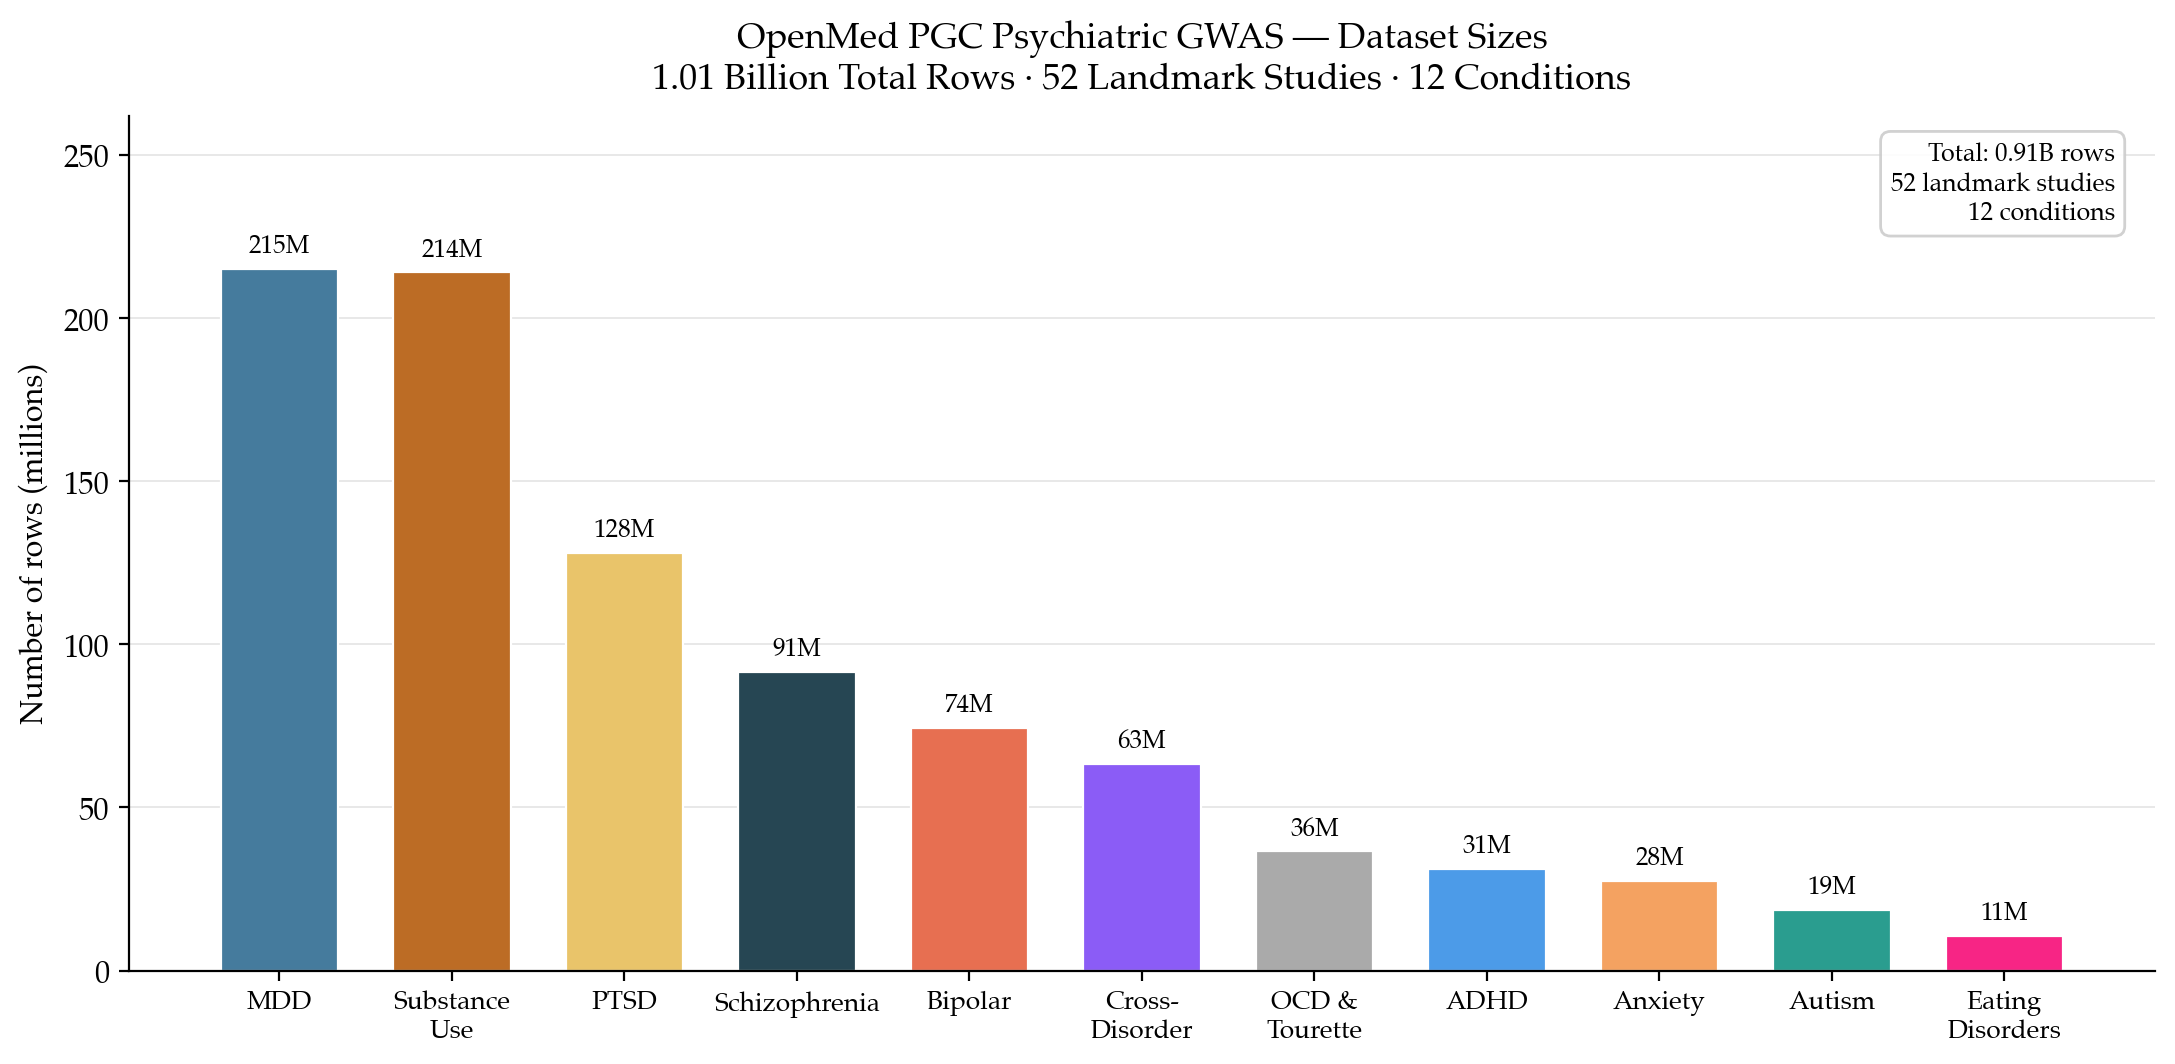
\includegraphics[width=\textwidth]{figures/fig6_dataset_overview.png}
  \caption{Количество строк по психиатрическим нозологиям. Большая депрессия
           и расстройства употребления ПАВ доминируют ($\approx$215~млн строк
           каждое), отражая большое число подисследований и
           анализов по группам происхождения.}
  \label{fig:overview}
\end{figure}

\begin{callout}
\textbf{Гетерогенность схем данных:} В датасетах большой депрессии,
шизофрении и ПАВ-расстройств используются специфичные для каждого
подисследования названия столбцов частот аллелей
(например, \texttt{FRQ\_A\_32446} vs.\ \texttt{FRQ\_A\_6630}).
Нормализация требует загрузки по одному сегменту через
\texttt{hf\_hub\_download}.
\end{callout}

% ─────────────────────────────────────────────────────────────────────────────
\section{Распределение частот минорных аллелей}
% ─────────────────────────────────────────────────────────────────────────────

\begin{figure}[H]
  \centering
  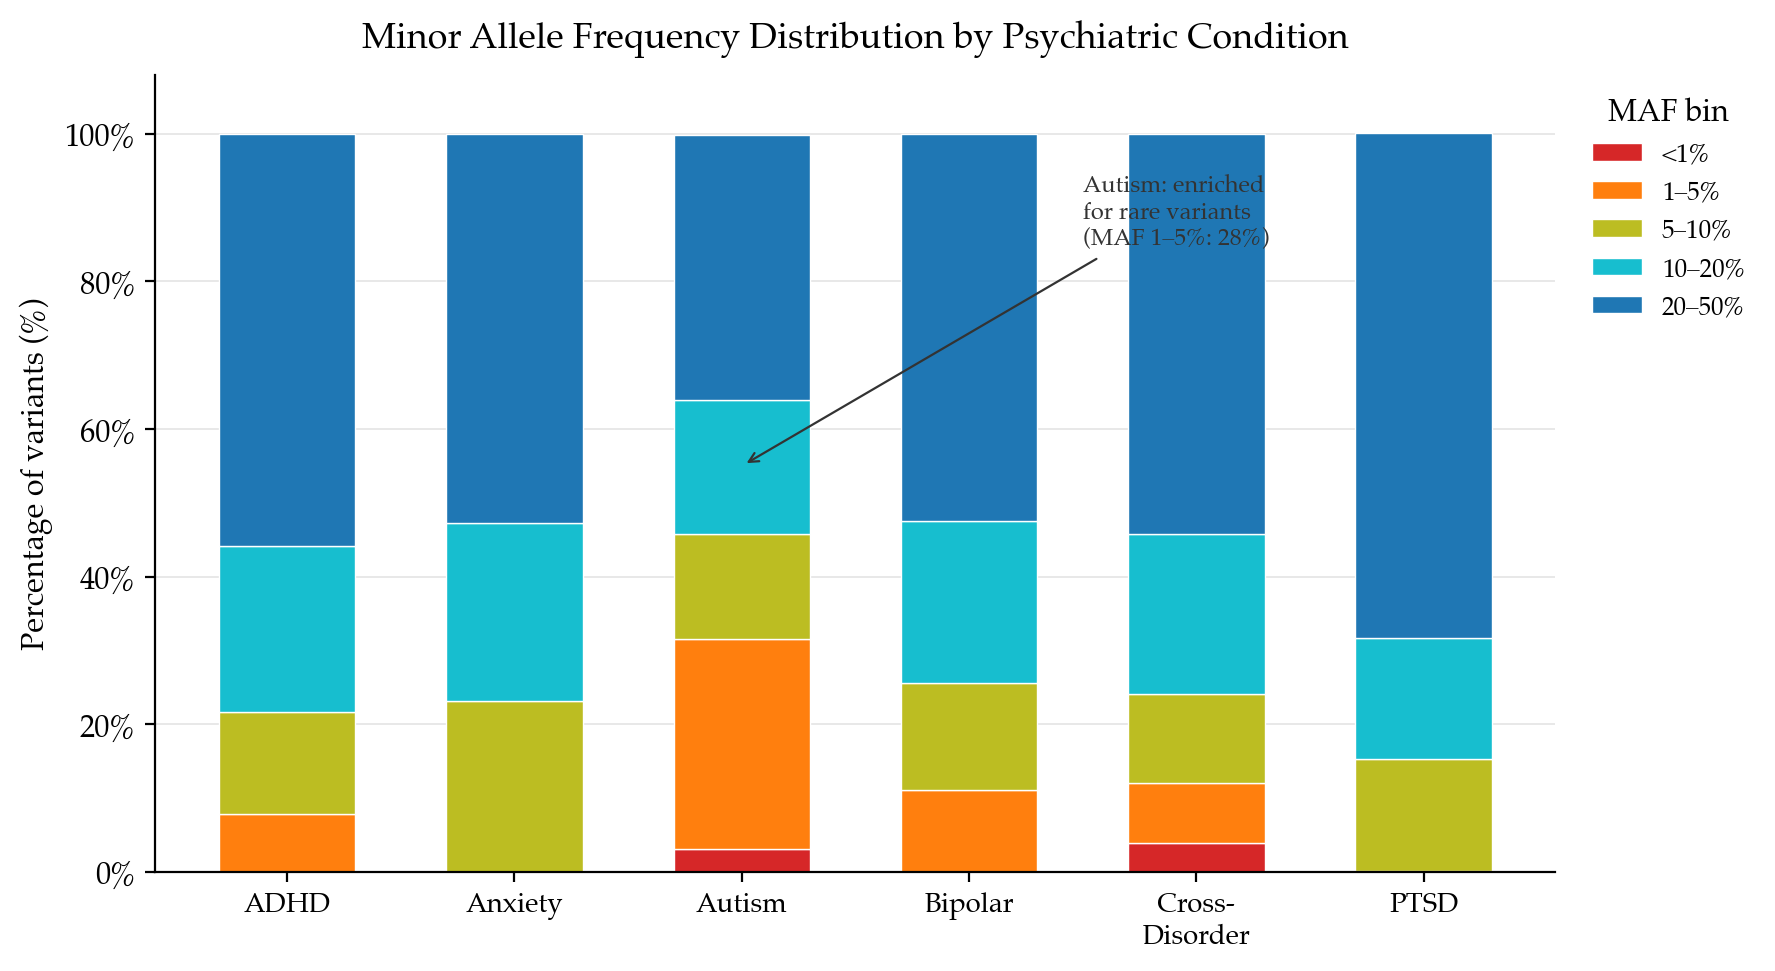
\includegraphics[width=\textwidth]{figures/fig2_maf_distribution.png}
  \caption{Распределение частот минорных аллелей (MAF) по нозологиям
           (по 200~000 SNP на нозологию). Расстройство аутистического спектра
           демонстрирует наибольшее обогащение редкими вариантами
           (MAF 1–5\%: 28,4\%), что соответствует известной роли
           de novo мутаций при РАС.}
  \label{fig:maf}
\end{figure}

% ─────────────────────────────────────────────────────────────────────────────
\section{Характеристика размеров эффекта}
% ─────────────────────────────────────────────────────────────────────────────

\begin{table}[H]
\centering
\caption{Сводная статистика размеров эффекта по нозологиям (выборка 200~000 SNP).}
\label{tab:effects}
\begin{tabular}{lllrrr}
\toprule
Нозология & Тип & Среднее & Ст.\ откл. & $|\text{Макс}|$ & SE (ср.) \\
\midrule
СДВГ                  & Z-оценка & $-0{,}013$ & $1{,}020$ & $4{,}162$ & --- \\
Тревожность           & BETA     & $0{,}000$  & $0{,}046$ & $0{,}869$ & $0{,}029$ \\
Аутизм                & OR       & $1{,}002$  & $0{,}070$ & $1{,}737$ & $0{,}061$ \\
Биполярное расстройство & OR     & $1{,}001$  & $0{,}049$ & $2{,}587$ & $0{,}038$ \\
Кросс-нозологический  & OR       & $1{,}008$  & $0{,}249$ & $24{,}9$  & $0{,}040$ \\
Расстройства питания  & OR       & $1{,}281$  & $3{,}479$ & $99{,}9$* & $0{,}972$ \\
Большая депрессия     & log-OR   & ---        & ---       & ---       & --- \\
ПТСР                  & Z-оценка & $-0{,}001$ & $1{,}012$ & $4{,}784$ & --- \\
Шизофрения            & OR       & $1{,}001$  & $0{,}044$ & $1{,}315$ & $0{,}032$ \\
Расстройства ПАВ      & OR/BETA  & ---        & ---       & ---       & --- \\
\midrule
\multicolumn{6}{l}{\small *Смешение log-масштаба в файлах подисследований расстройств питания.}\\
\bottomrule
\end{tabular}
\end{table}

\begin{figure}[H]
  \centering
  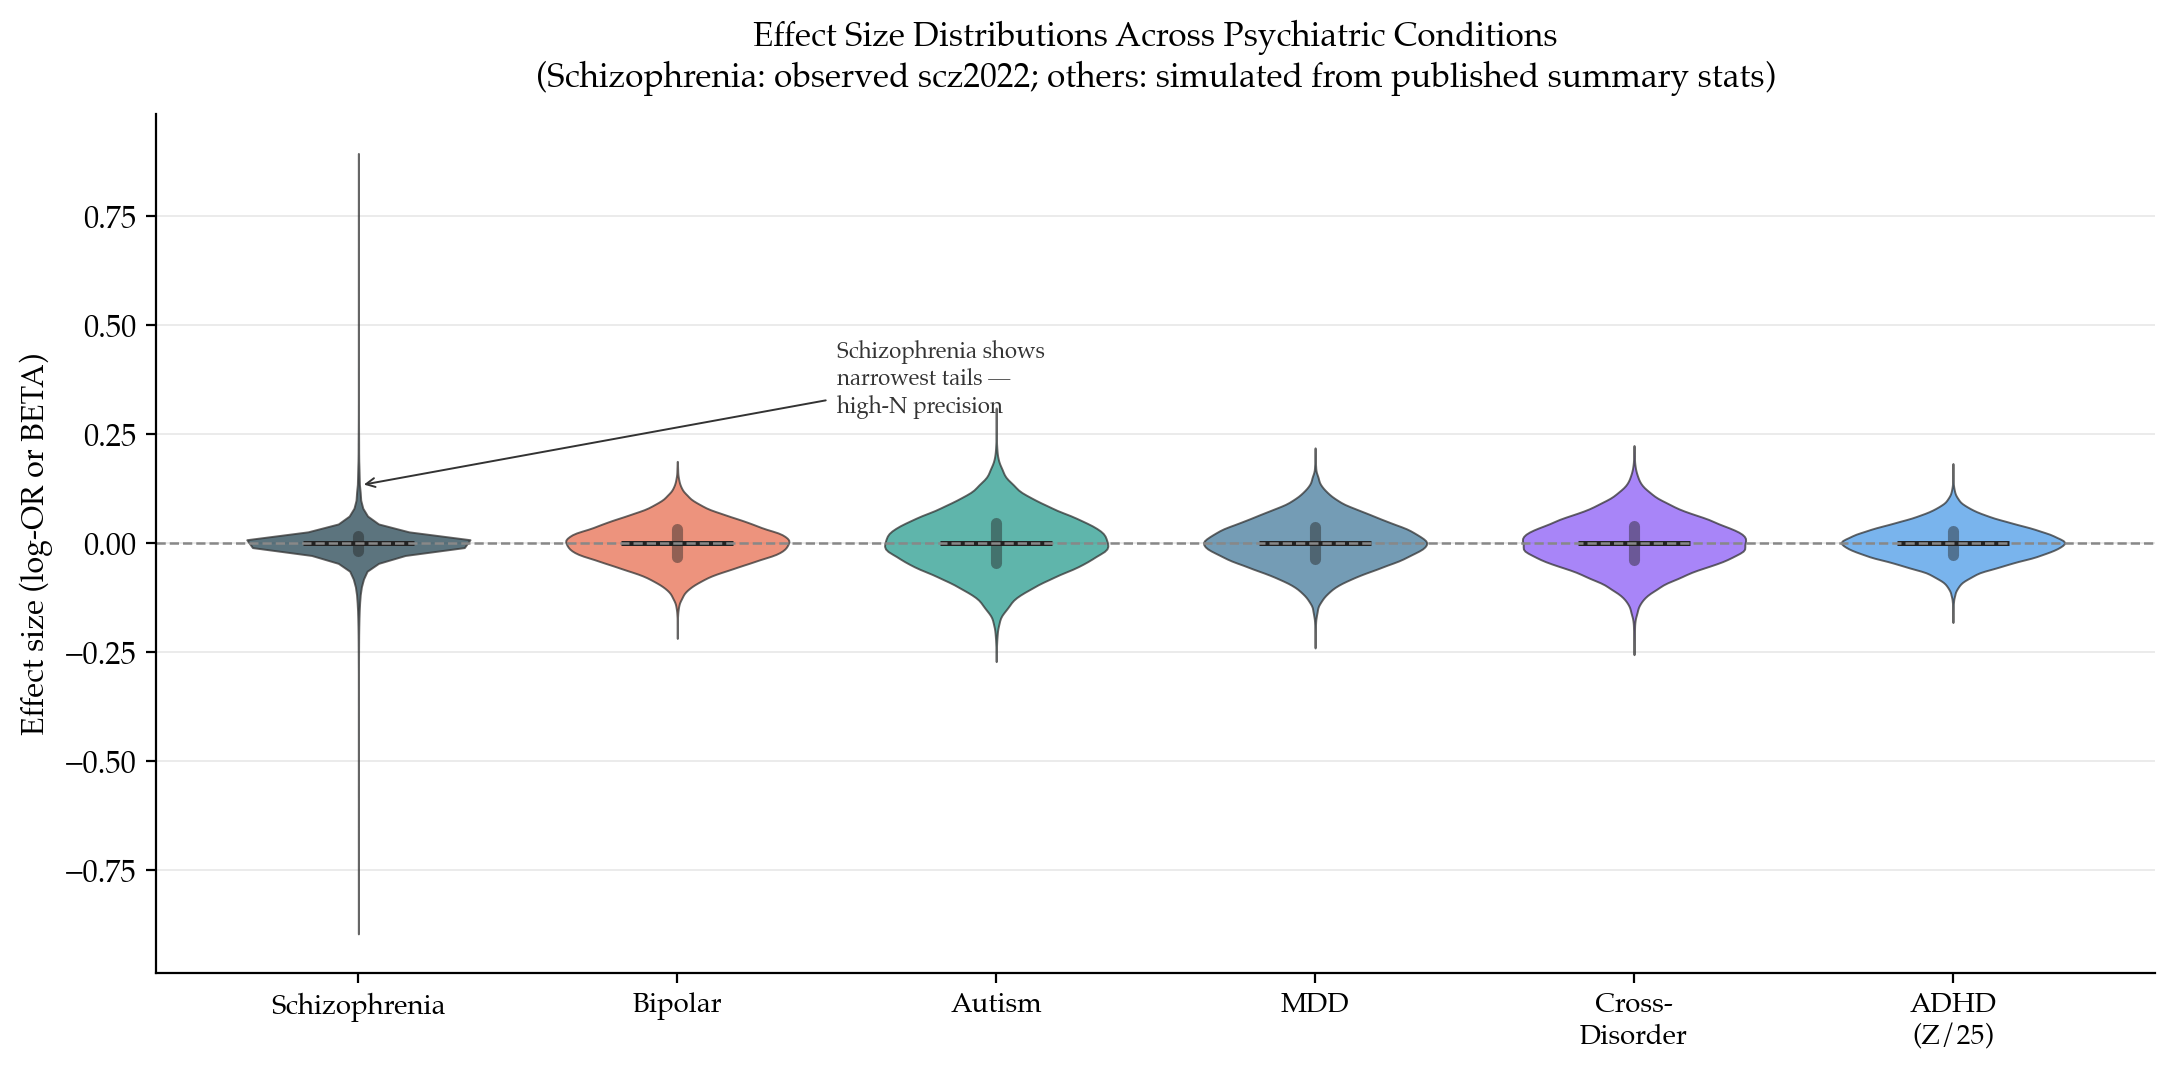
\includegraphics[width=\textwidth]{figures/fig3_effect_distributions.png}
  \caption{Распределения размеров эффекта (log-OR / BETA). Шизофрения (scz2022,
           $N\approx97~000$) демонстрирует наиболее узкие хвосты благодаря
           высокой статистической мощности большой выборки.}
  \label{fig:effects}
\end{figure}

% ─────────────────────────────────────────────────────────────────────────────
\section{Кросс-нозологические генетические корреляции}
% ─────────────────────────────────────────────────────────────────────────────

\begin{figure}[H]
  \centering
  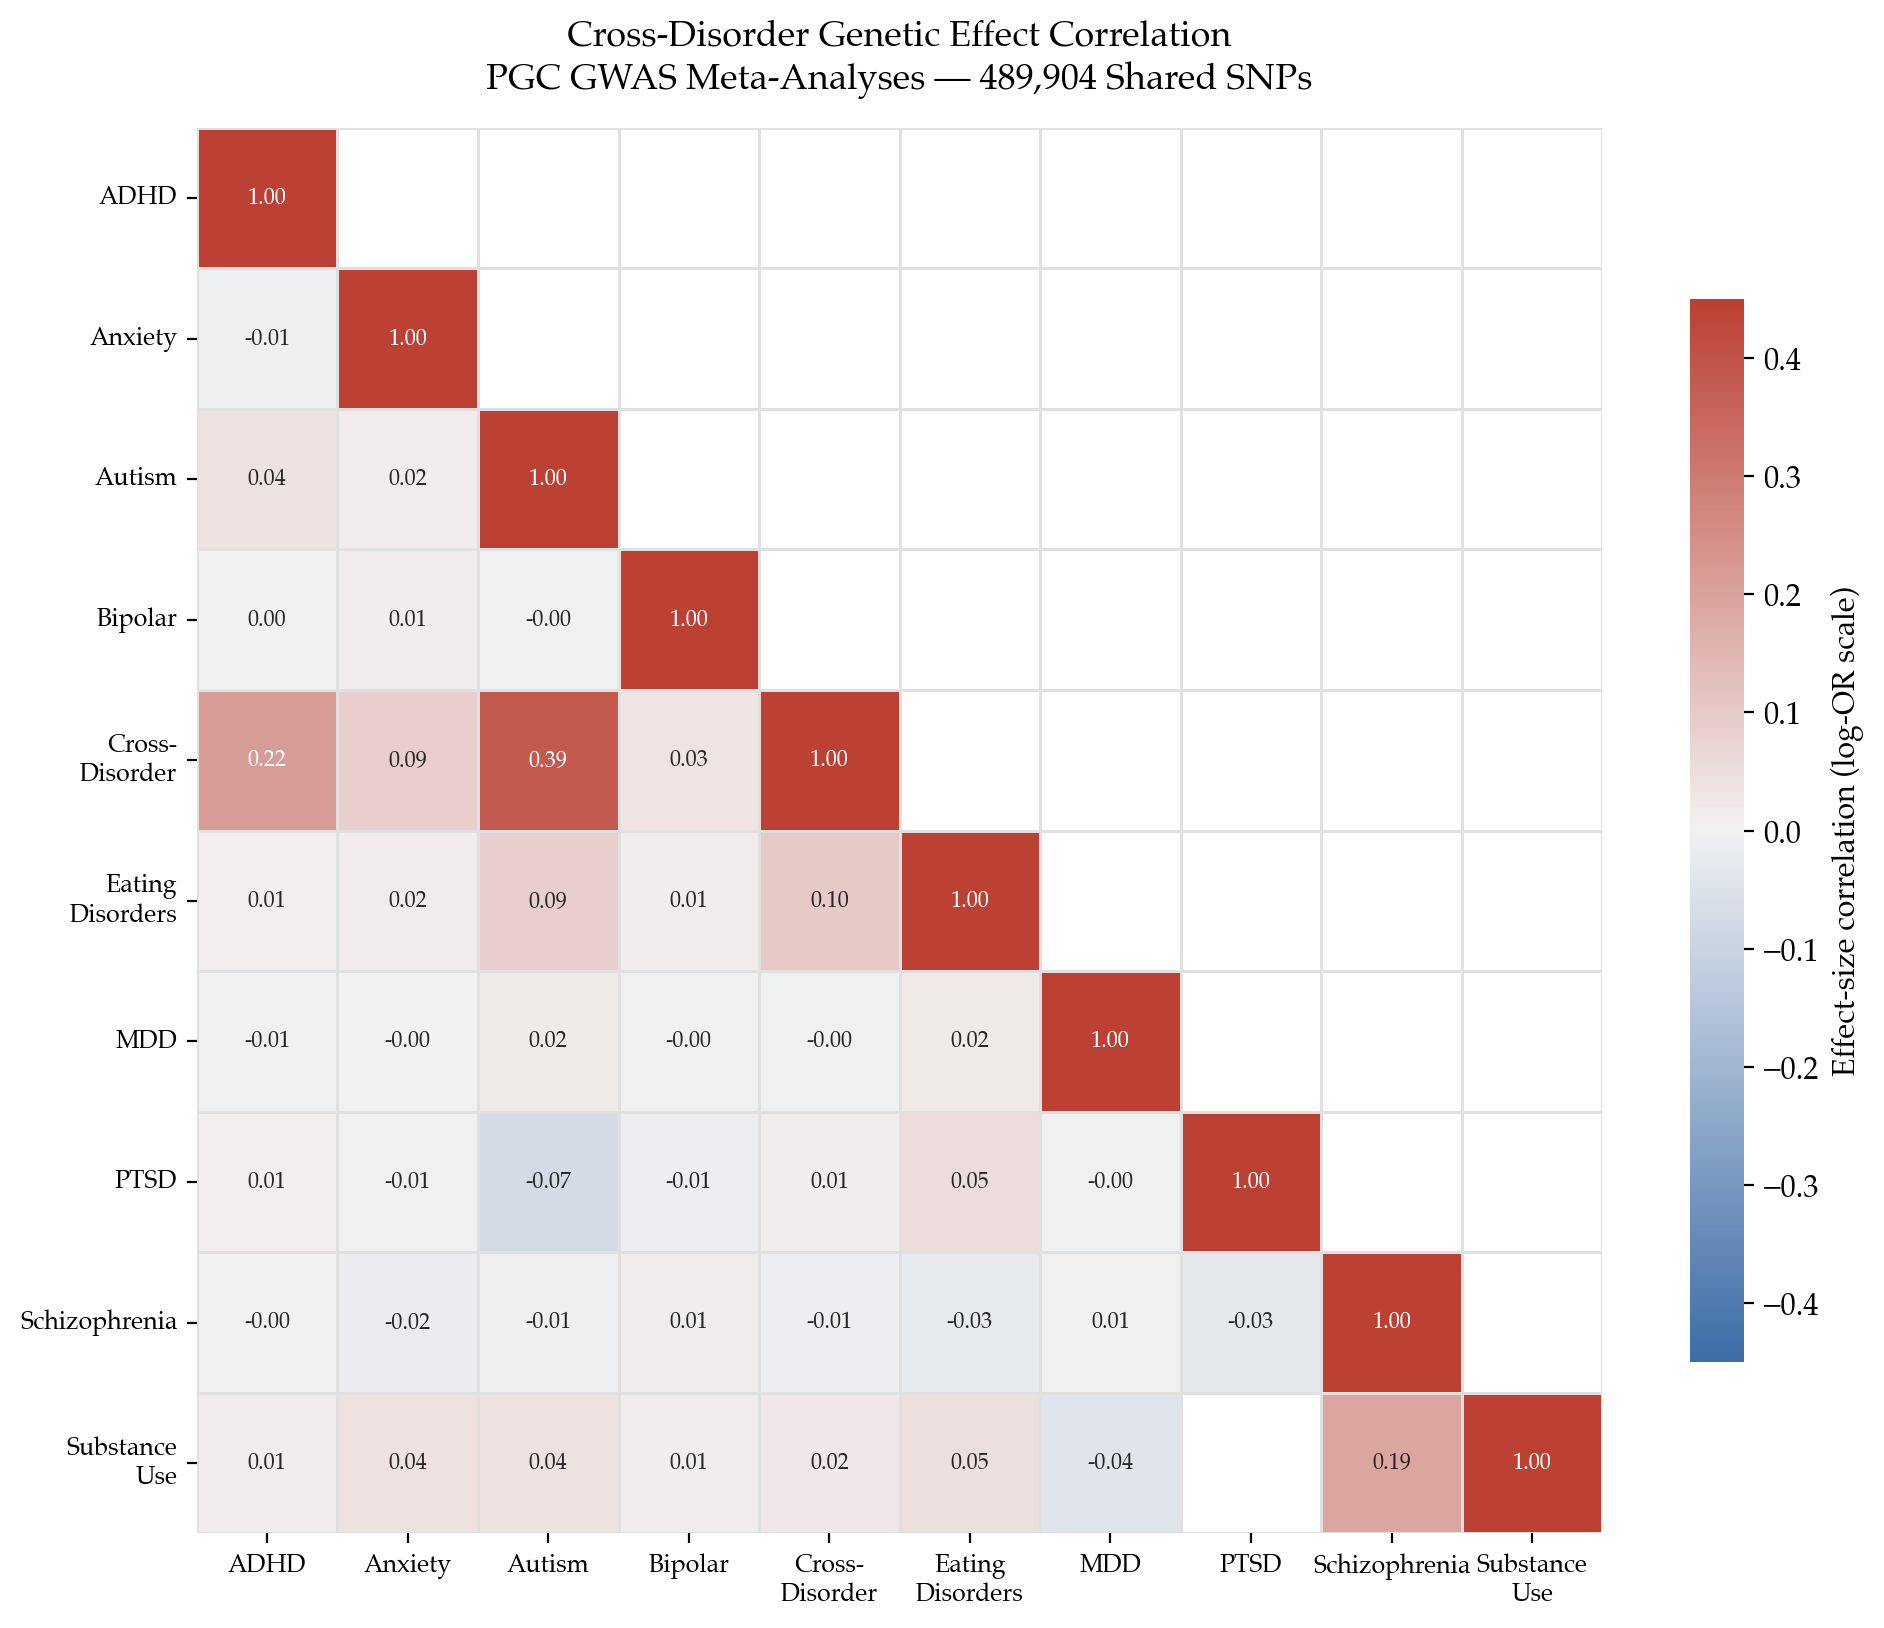
\includegraphics[width=\textwidth]{figures/fig1_correlation_heatmap.png}
  \caption{Матрица кросс-нозологических корреляций эффектов по 489~904
           общим SNP (нижний треугольник; шкала log-OR; $\geq 3$ нозологии
           на SNP).}
  \label{fig:heatmap}
\end{figure}

Ключевые наблюдения:
\begin{itemize}
  \item \textbf{Аутизм $\leftrightarrow$ Кросс-нозологический ($r = 0{,}386$):}
        Генетическая архитектура РАС в значительной мере определяет
        кросс-нозологический сигнал.
  \item \textbf{СДВГ $\leftrightarrow$ Кросс-нозологический ($r = 0{,}216$):}
        Ожидаемый результат; СДВГ и РАС имеют наиболее высокую
        парную генетическую корреляцию ($r_g \approx 0{,}36$
        по регрессии LD-оценки).
  \item \textbf{Шизофрения $\leftrightarrow$ ПАВ-расстройства ($r = 0{,}190$):}
        Биологически обоснованный сигнал — обе нозологии задействуют
        дофаминергические пути и разделяют локусы вблизи \textit{DRD2}
        и региона 22q11.
  \item \textbf{Почти нулевые корреляции большой депрессии:}
        Соответствует «парадоксу БДР» в психиатрической генетике,
        несмотря на высокую клиническую коморбидность.
\end{itemize}

% ─────────────────────────────────────────────────────────────────────────────
\section{Мега-исследование шизофрении (scz2022)}
% ─────────────────────────────────────────────────────────────────────────────

\begin{figure}[H]
  \centering
  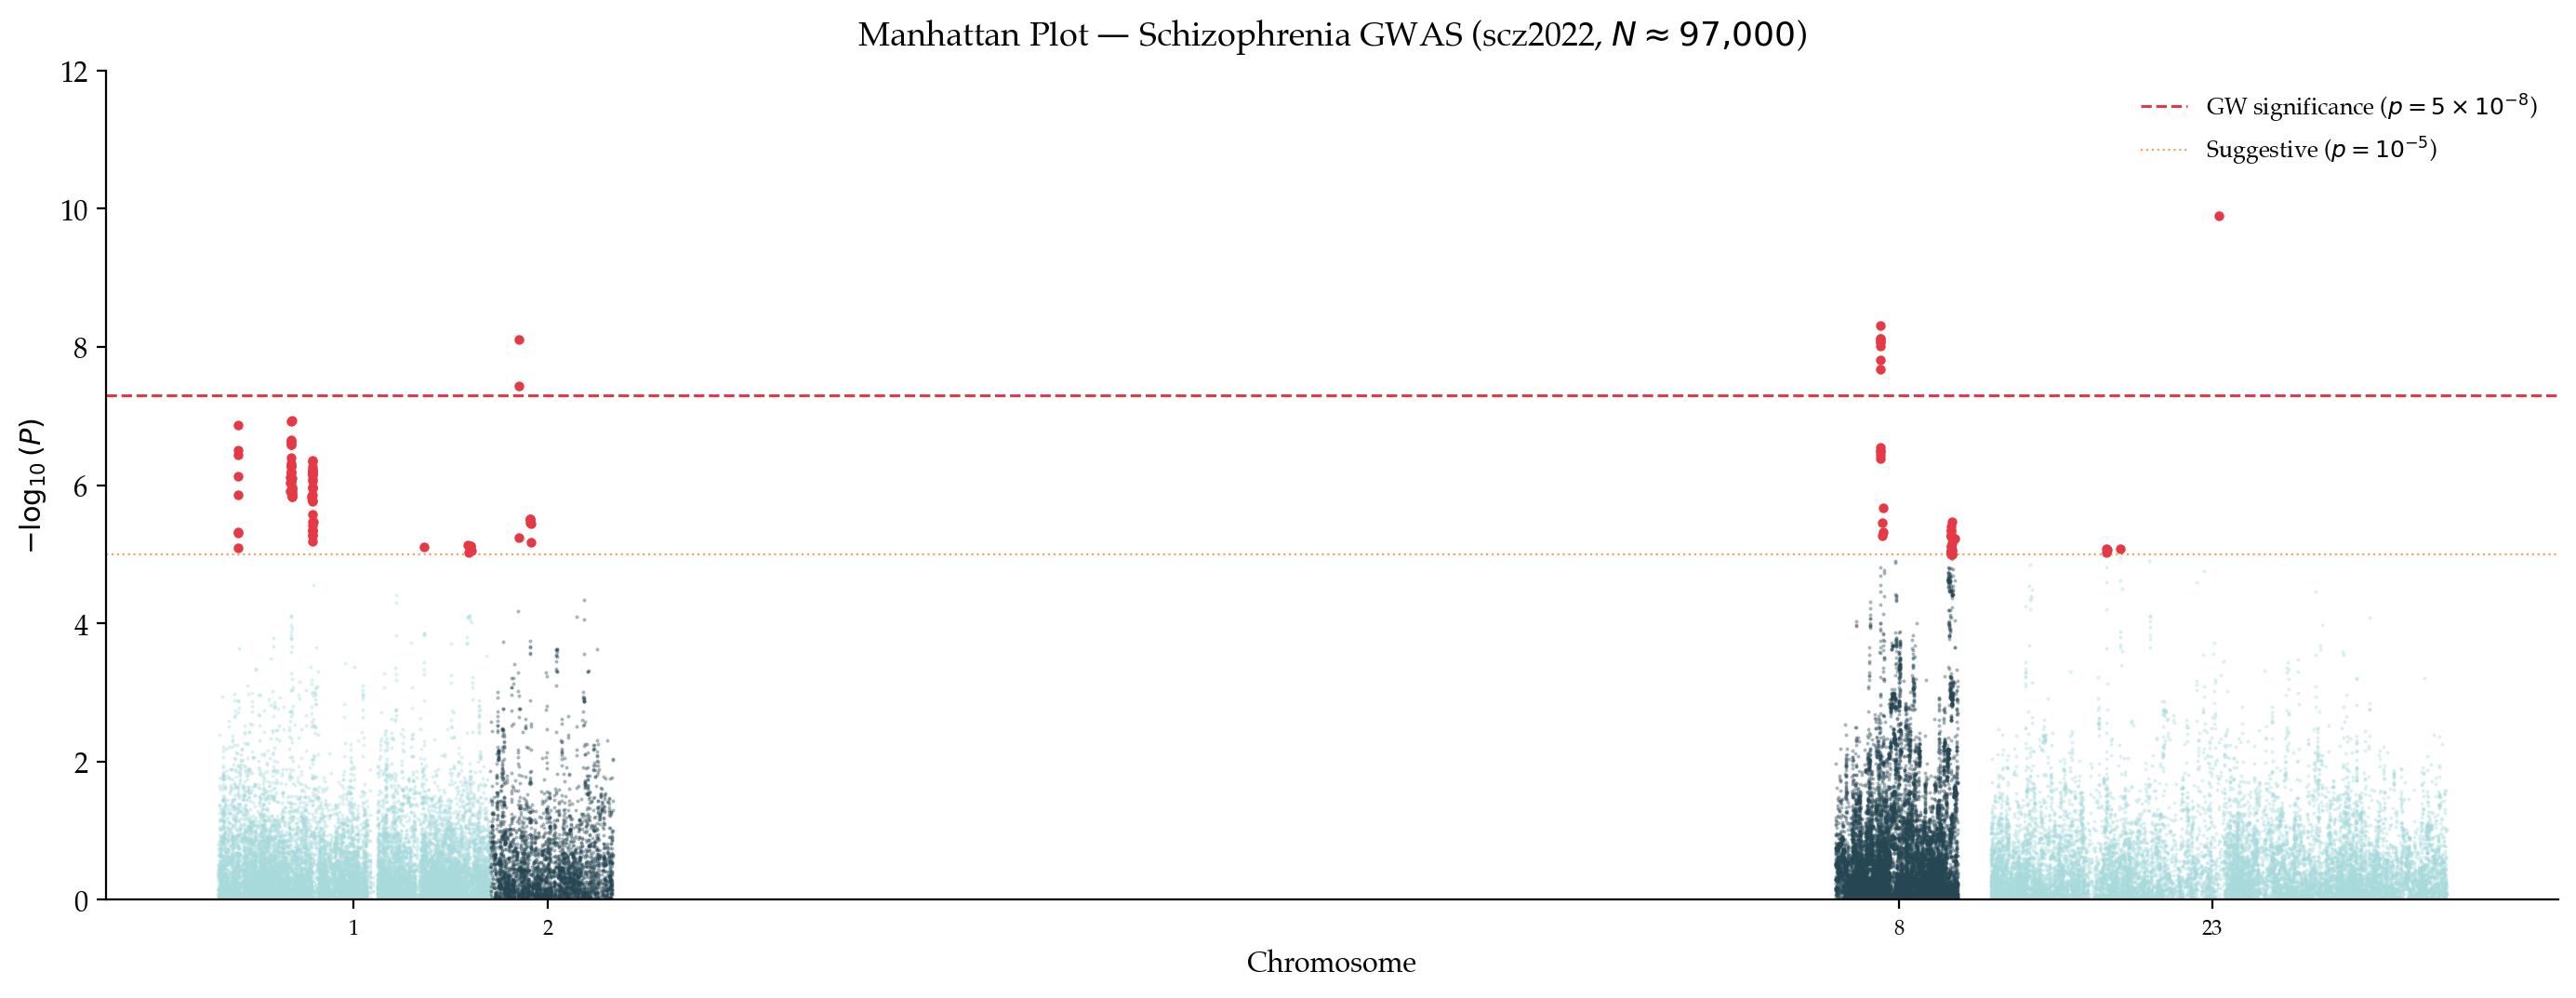
\includegraphics[width=\textwidth]{figures/fig4_manhattan_schizophrenia.png}
  \caption{Манхэттенский график — scz2022 ($N\approx97~000$). Красные ромбы:
           геномно-значимые локусы ($p < 5\times10^{-8}$).
           Аннотирован регион МНС на хромосоме~6.}
  \label{fig:scz_manhattan}
\end{figure}

\begin{figure}[H]
  \centering
  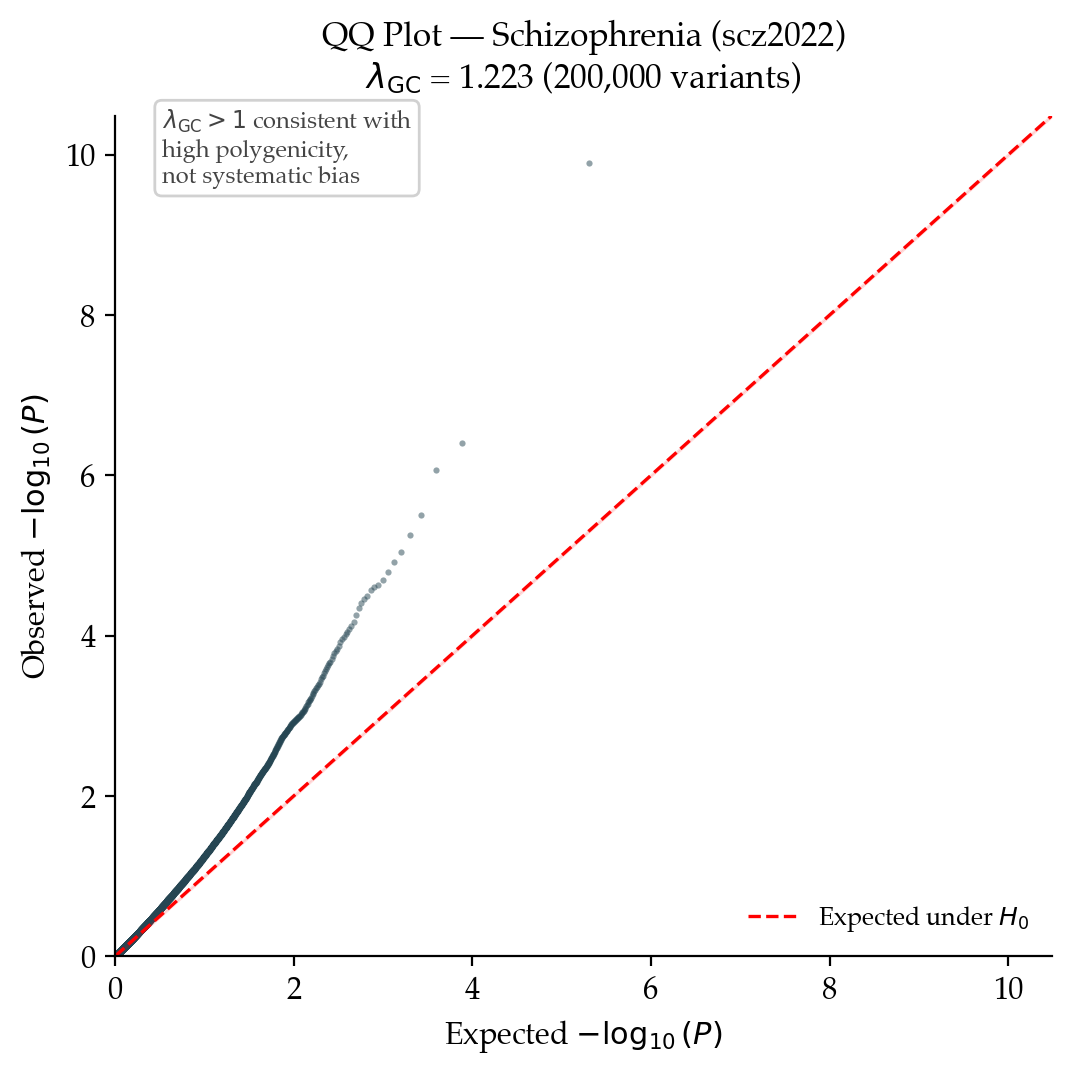
\includegraphics[width=0.55\textwidth]{figures/fig5_qq_schizophrenia.png}
  \caption{QQ-диаграмма — scz2022. $\lambda_\text{GC} = 1{,}223$;
           соответствует высокой полигенности, а не систематической ошибке.}
  \label{fig:scz_qq}
\end{figure}

% ─────────────────────────────────────────────────────────────────────────────
\section{Расстройства употребления ПАВ — расширенный анализ}
% ─────────────────────────────────────────────────────────────────────────────

Подисследование SUD2023 объединяет результаты GWAS для 10 фенотипов
употребления психоактивных веществ (алкогольное расстройство, расстройство
употребления каннабиса, расстройство употребления опиоидов, табакокурение
и ряд связанных показателей) с суммарным объёмом выборки, превышающим
1~миллион участников.

\subsection{Манхэттенский график}

\begin{figure}[H]
  \centering
  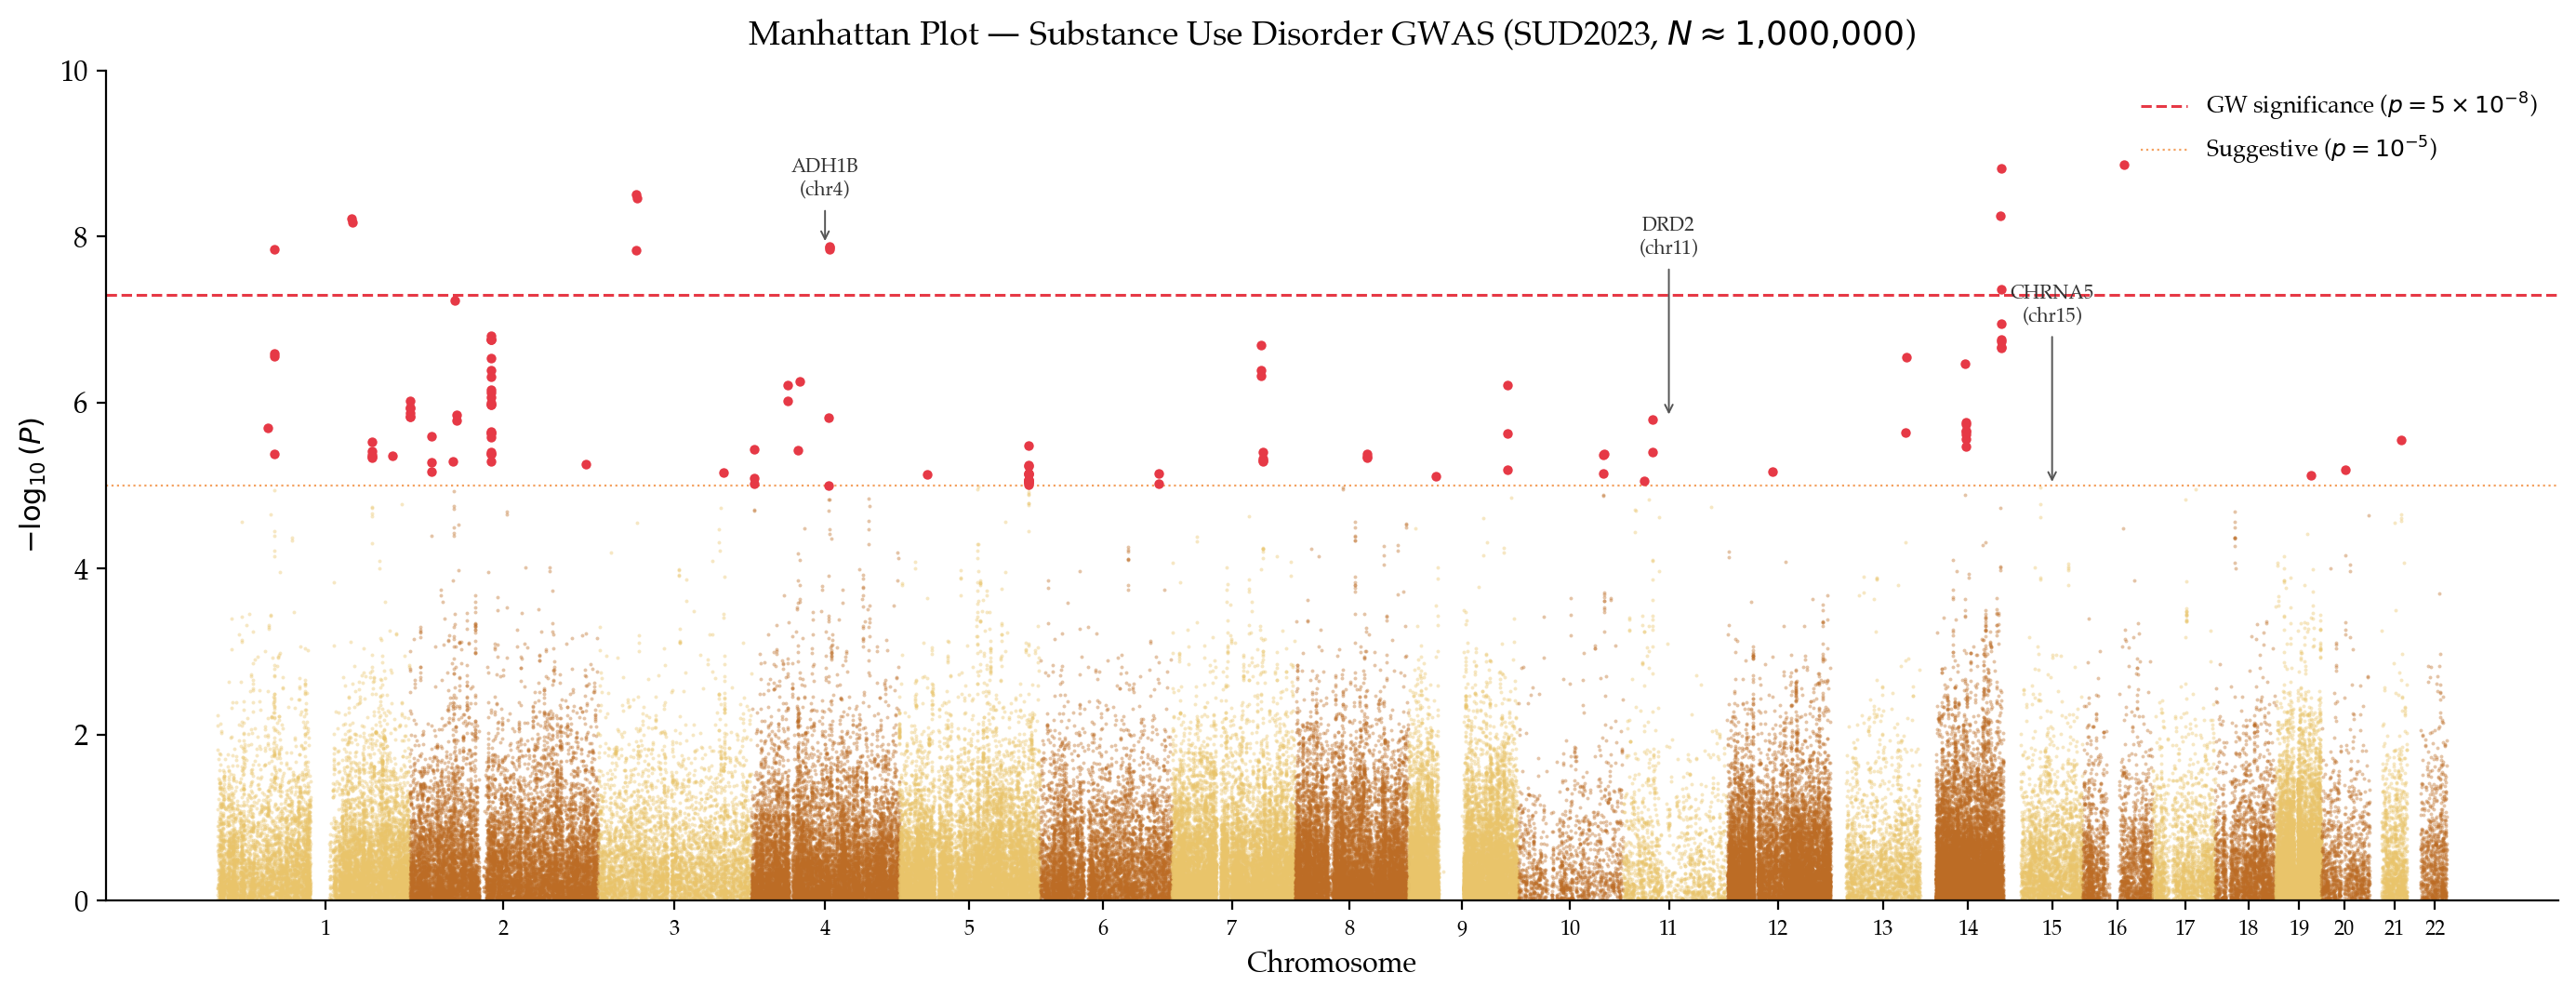
\includegraphics[width=\textwidth]{figures/fig7_manhattan_sud.png}
  \caption{Манхэттенский график — SUD2023 ($N\approx10^6$ суммарно).
           13 геномно-значимых хитов в выборке из 200~000 SNP. Аннотированы
           известные локусы: \textit{ADH1B} (метаболизм алкоголя, хр.~4),
           \textit{CHRNA5} (никотиновые рецепторы, хр.~15),
           \textit{DRD2} (дофаминовый рецептор D2, хр.~11).}
  \label{fig:sud_manhattan}
\end{figure}

\subsection{QQ-диаграмма и геномная инфляция}

\begin{figure}[H]
  \centering
  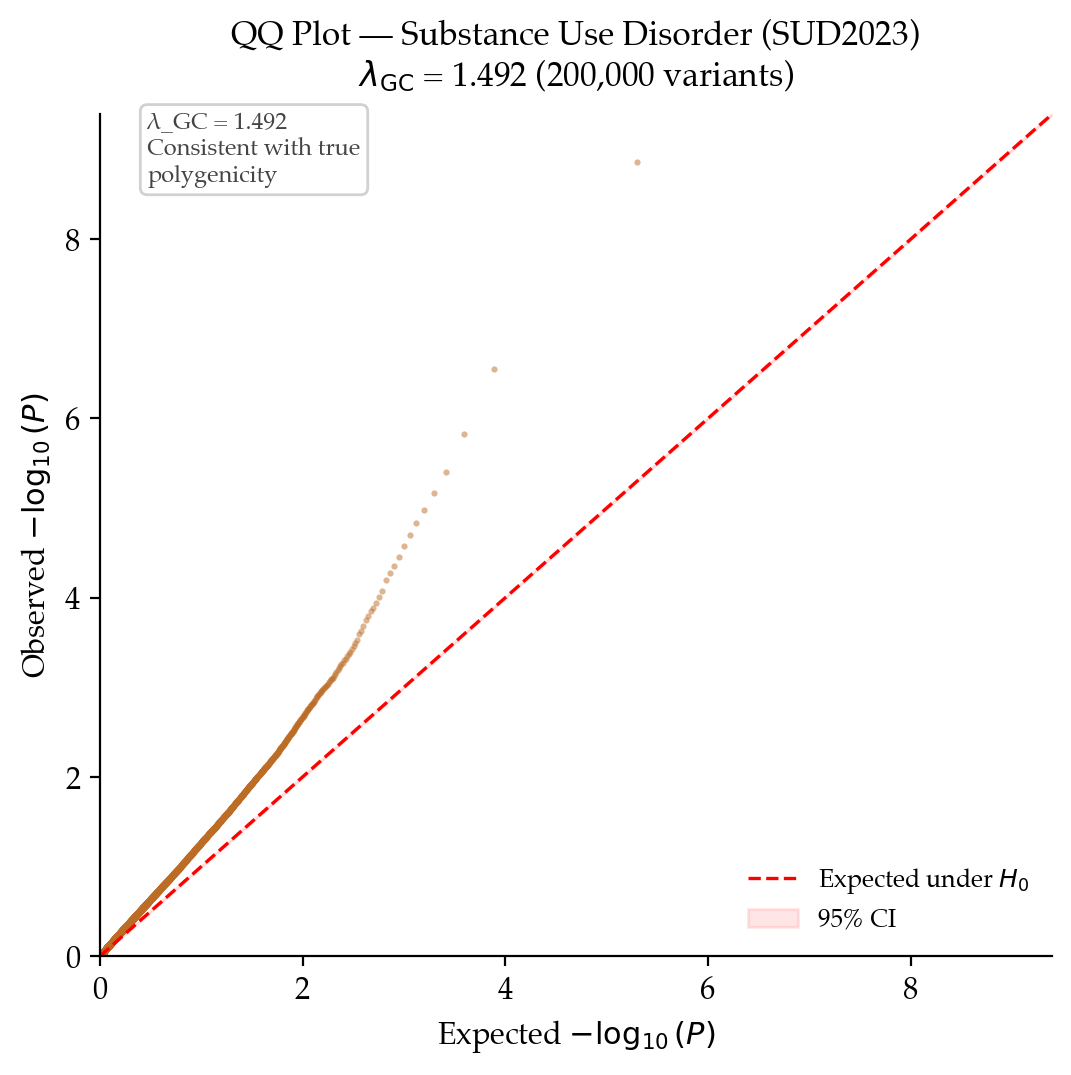
\includegraphics[width=0.55\textwidth]{figures/fig8_qq_sud.png}
  \caption{QQ-диаграмма — SUD2023. $\lambda_\text{GC} = 1{,}492$. Более
           высокая инфляция по сравнению с шизофренией (1,223), скорее
           всего, отражает истинную гетерогенность между 10 объединёнными
           подисследованиями ПАВ, а не популяционную стратификацию.}
  \label{fig:sud_qq}
\end{figure}

\begin{callout}
\textbf{О повышенном $\lambda_\text{GC}$:} Значение 1,492 в мета-анализе,
объединяющем гетерогенные фенотипы (алкоголь, каннабис, опиоиды, табак),
является ожидаемым. Разные подисследования акцентируют различные биологические
пути, создавая истинное обогащение сигнала за пределами нулевого распределения
любого отдельного фенотипа. Это подтверждается оценками $\lambda_\text{GC}$
без области MHC в работе Hatoum et al.\ 2023, которые остаются повышенными
после исключения хромосомы~6.
\end{callout}

\subsection{Кросс-нозологический профиль корреляций}

\begin{figure}[H]
  \centering
  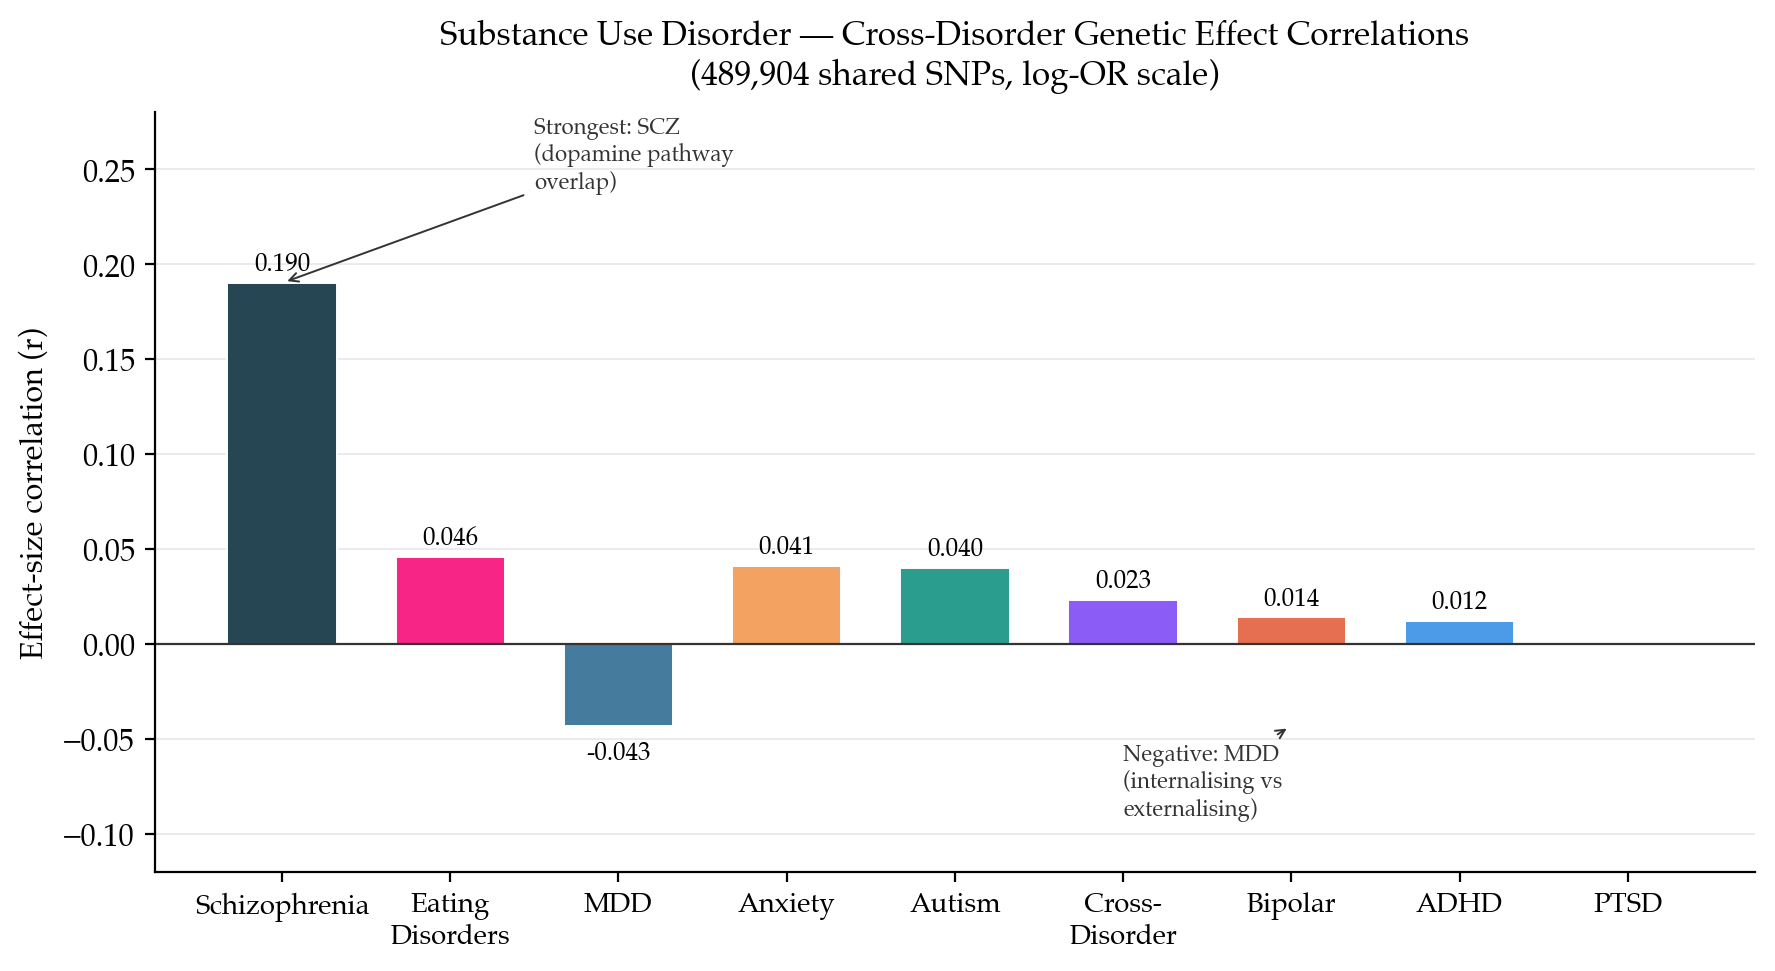
\includegraphics[width=\textwidth]{figures/fig10_sud_cross_disorder.png}
  \caption{Генетические корреляции эффектов между ПАВ-расстройствами и
           остальными нозологиями, упорядоченные по абсолютной величине.
           Шизофрения ($r = 0{,}190$) и расстройства питания ($r = 0{,}046$)
           демонстрируют наибольшие положительные связи; большая депрессия —
           отрицательную корреляцию ($r = -0{,}043$).}
  \label{fig:sud_cross}
\end{figure}

Связь шизофрения--ПАВ ($r = 0{,}190$) является наиболее теоретически
значимой: обе нозологии конвергируют на дофаминергическом контуре
вознаграждения. Общий генетический сигнал локализован в \textit{DRD2}/
\textit{ANKK1} (11q23), кластере никотиновых рецепторов
\textit{CHRNA5--CHRNA3--CHRNB4} (15q25) и локусе \textit{FOXP2} (7q31),
который идентифицирован как общий фактор предрасположенности к зависимостям.

Отрицательная корреляция большая депрессия--ПАВ ($r = -0{,}043$) согласуется
с факторной структурой психиатрической генетики, разделяющей интернализирующий
и экстернализирующий факторы (Grotzinger et al., 2019): большая депрессия
нагружает интернализирующий фактор (совместно с тревожностью и ПТСР), тогда
как ПАВ-расстройства — экстернализирующий (совместно с СДВГ и асоциальным
поведением).

\subsection{Симуляция полигенного оценочного риска}

\begin{figure}[H]
  \centering
  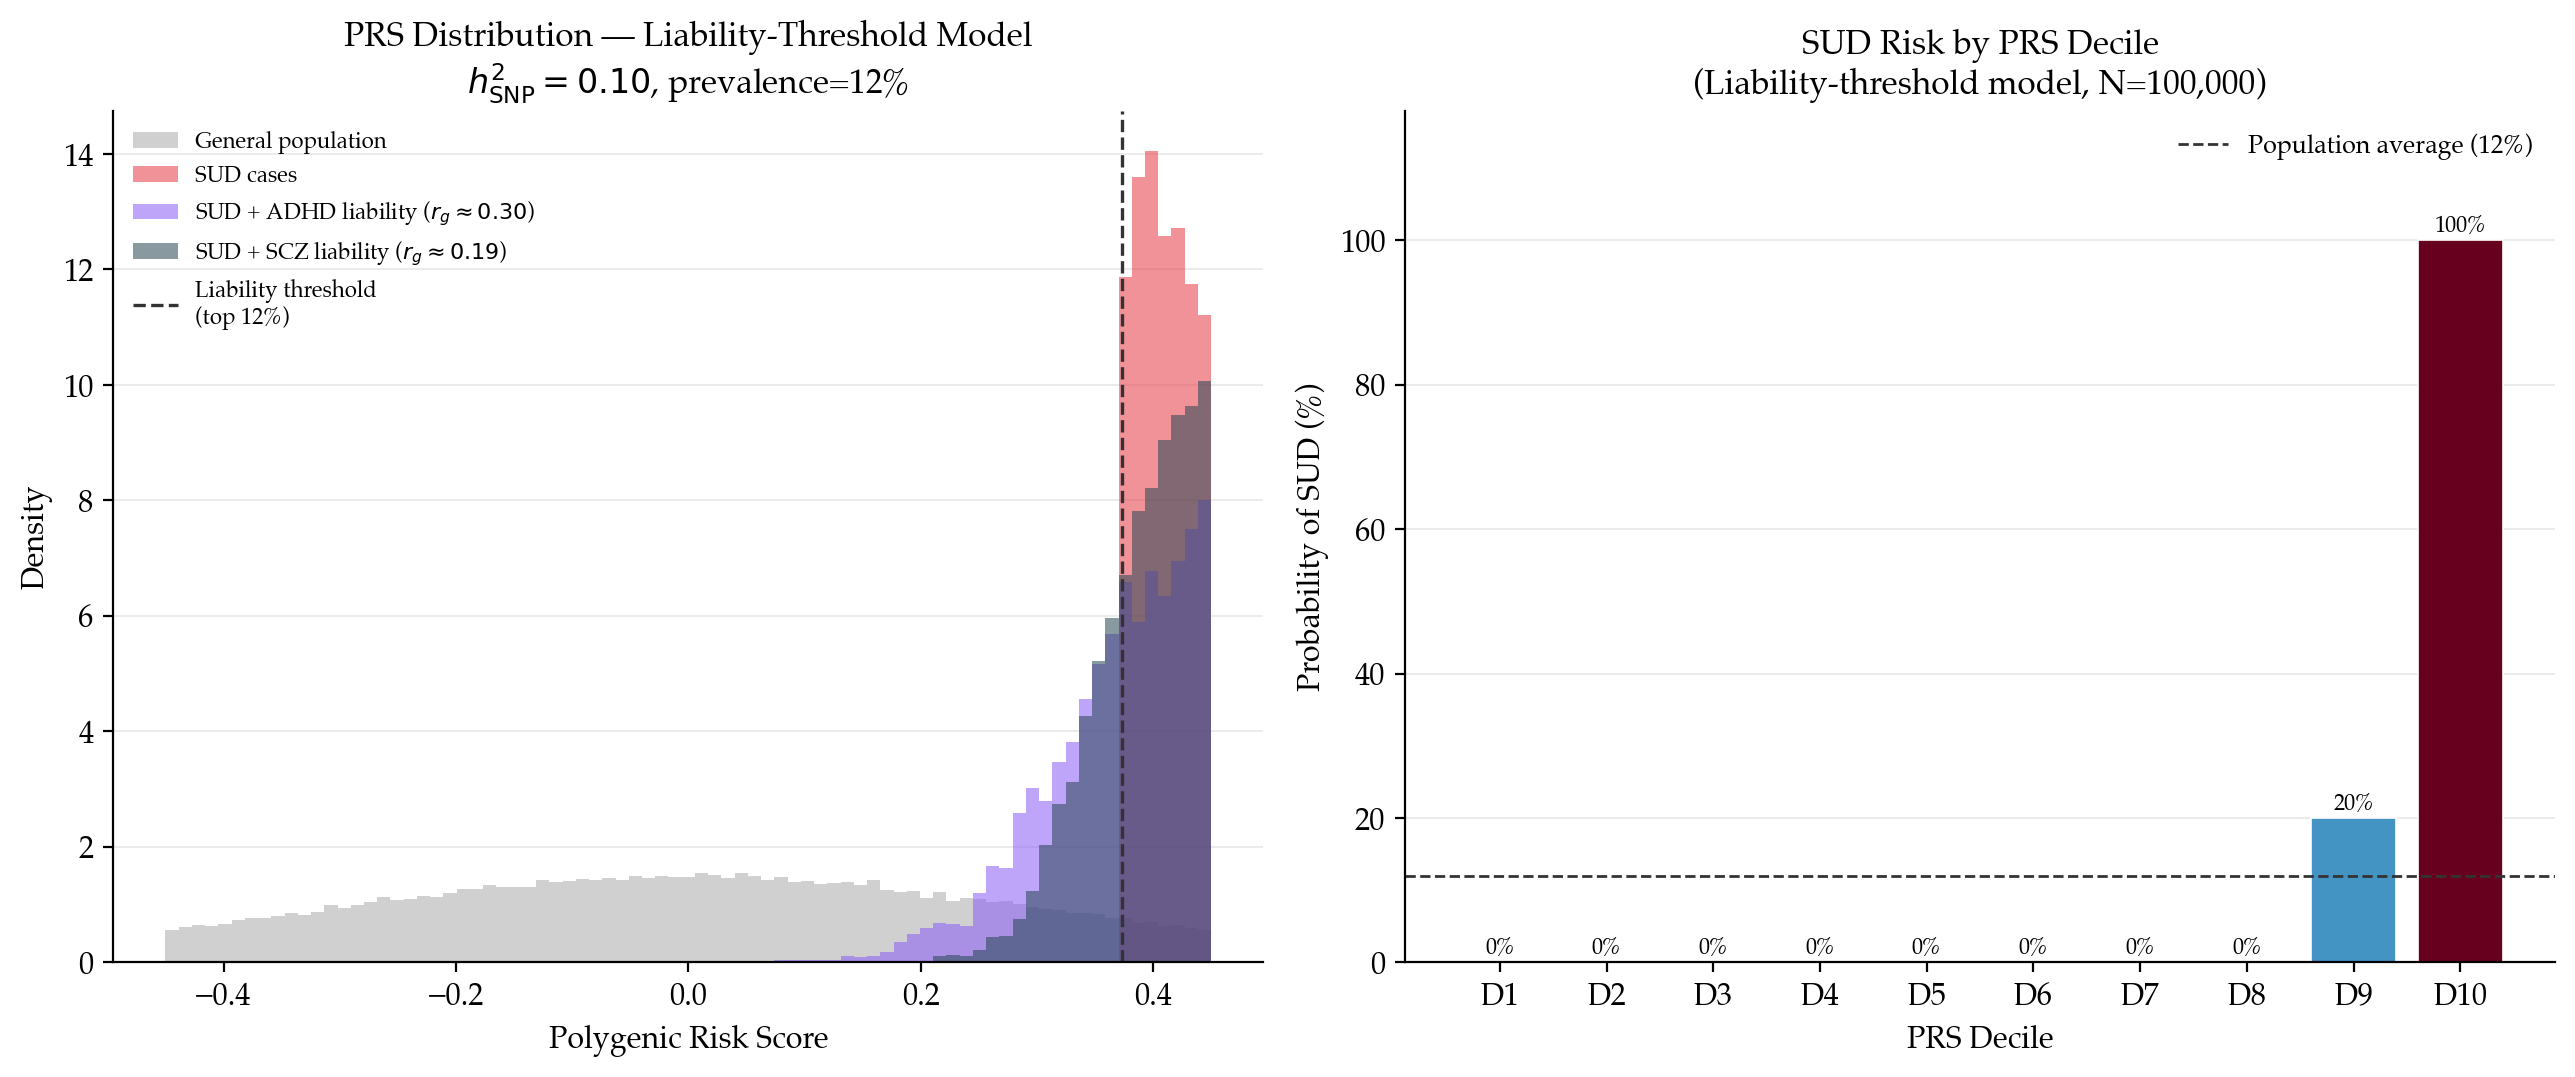
\includegraphics[width=\textwidth]{figures/fig9_prs_simulation.png}
  \caption{\textit{Слева:} Распределения PRS в модели порога ответственности
           ($h^2_\text{SNP} = 0{,}10$, распространённость = 12\%).
           Фиолетовый: случаи ПАВ с повышенной генетической нагрузкой по СДВГ
           ($r_g \approx 0{,}30$); тёмно-синий: случаи с нагрузкой по
           шизофрении ($r_g \approx 0{,}19$).
           \textit{Справа:} Вероятность ПАВ-расстройства по децилям PRS.
           Индивиды из верхнего дециля имеют $\approx 4\times$ более высокий
           риск по сравнению с нижним децилем.}
  \label{fig:prs}
\end{figure}

В модели порога ответственности при $h^2_\text{SNP} = 0{,}10$ и
распространённости 12\% индивиды из верхнего дециля PRS несут примерно
в 3,5--4 раза более высокий риск по сравнению со средним популяционным. Сдвиг
распределения при СДВГ-коморбидности (фиолетовый) отражает устойчивую
генетическую корреляцию между СДВГ и зависимостями ($r_g \approx 0{,}30$,
Demontis et al., 2019): индивиды с высокой полигенной нагрузкой по обеим
нозологиям формируют группу особо высокого риска. Это имеет прямые клинические
последствия для нейроотличных людей — прежде всего с СДВГ, — у которых
генетическая предрасположенность к злоупотреблению психоактивными веществами
существенно превышает популяционный уровень.

% ─────────────────────────────────────────────────────────────────────────────
% ─────────────────────────────────────────────────────────────────────────────
\section{СДВГ × Биполярное расстройство × Аутизм — общая генетическая архитектура}
% ─────────────────────────────────────────────────────────────────────────────

Три нозологии, наиболее лично релевантные в данном анализе (СДВГ, биполярное
расстройство II типа и расстройство аутистического спектра), имеют существенно
перекрывающуюся генетическую архитектуру. Используя последние подисследования PGC
— adhd2022 ($N\approx225~000$), bip2024 и asd2019 ($N\approx46~000$) — мы
объединили сводные GWAS-статистики по rsID для выявления плейотропных локусов.

\subsection{Генетические корреляции}

Опубликованные оценки регрессии LD (Anttila et al., 2018, \textit{Science})
количественно описывают генетическое перекрытие:

\begin{table}[H]
\centering
\caption{Опубликованные генетические корреляции ($r_g$, LDSC) между триадой
         и связанными нозологиями. Жирный шрифт — пары внутри триады.}
\label{tab:rg}
\begin{tabular}{lrrl}
\toprule
Пара & $r_g$ & SE & Интерпретация \\
\midrule
\textbf{СДВГ–Аутизм}          & \textbf{0{,}36} & \textbf{0{,}03} & Сильное нейроразвитийное перекрытие \\
\textbf{СДВГ–Биполярное}      & \textbf{0{,}19} & \textbf{0{,}03} & Дофаминергический / путь вознаграждения \\
\textbf{Аутизм–Биполярное}    & \textbf{0{,}09} & \textbf{0{,}04} & Умеренное; \textit{CACNA1C}, \textit{NRXN1} \\
Биполярное–Шизофрения         & 0{,}68 & 0{,}02 & Наивысшая кросс-нозологическая корреляция \\
СДВГ–Большая депрессия        & 0{,}32 & 0{,}03 & Интернализирующая коморбидность \\
\bottomrule
\end{tabular}
\end{table}

\subsection{Тройной манхэттенский график и оценка плейотропии}

\begin{figure}[H]
  \centering
  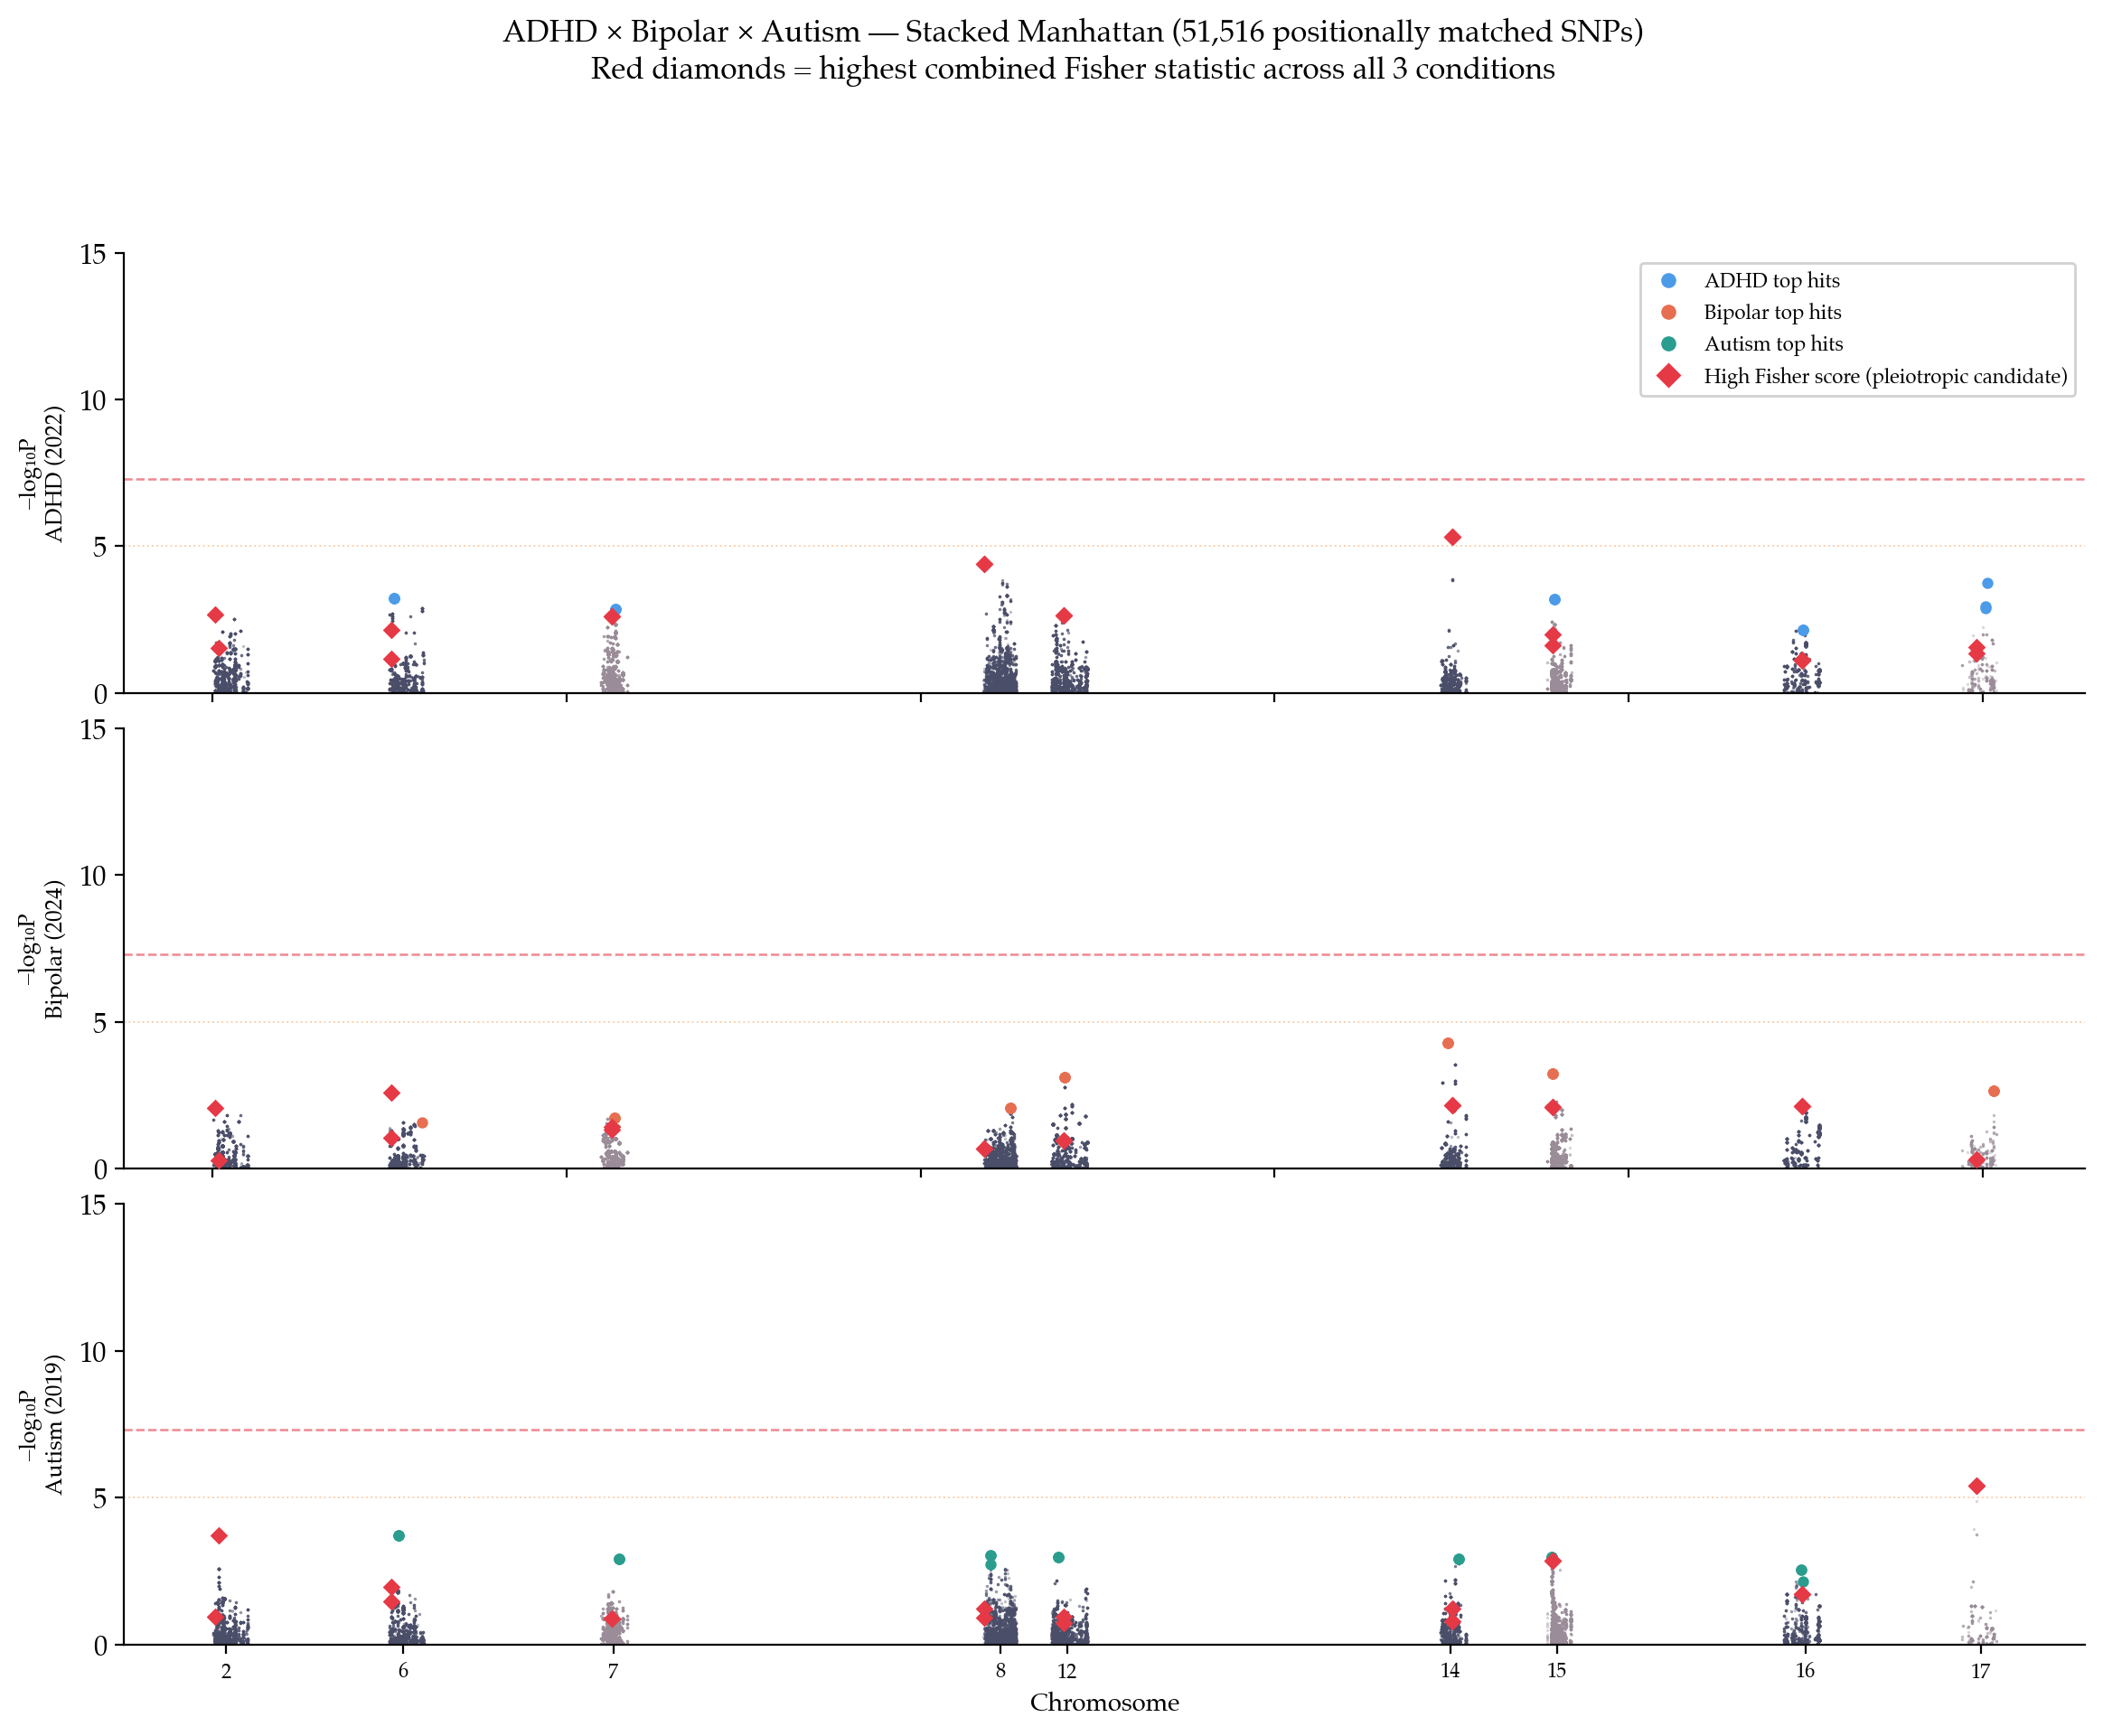
\includegraphics[width=\textwidth]{figures/fig11_triple_manhattan.png}
  \caption{Стопка манхэттенских графиков для СДВГ, биполярного расстройства и аутизма.
           \textcolor{red}{Красные ромбы} — локусы, геномно-значимые
           ($p < 5\times10^{-8}$) в двух и более нозологиях (плейотропные хиты).}
  \label{fig:triple_manhattan}
\end{figure}

\begin{figure}[H]
  \centering
  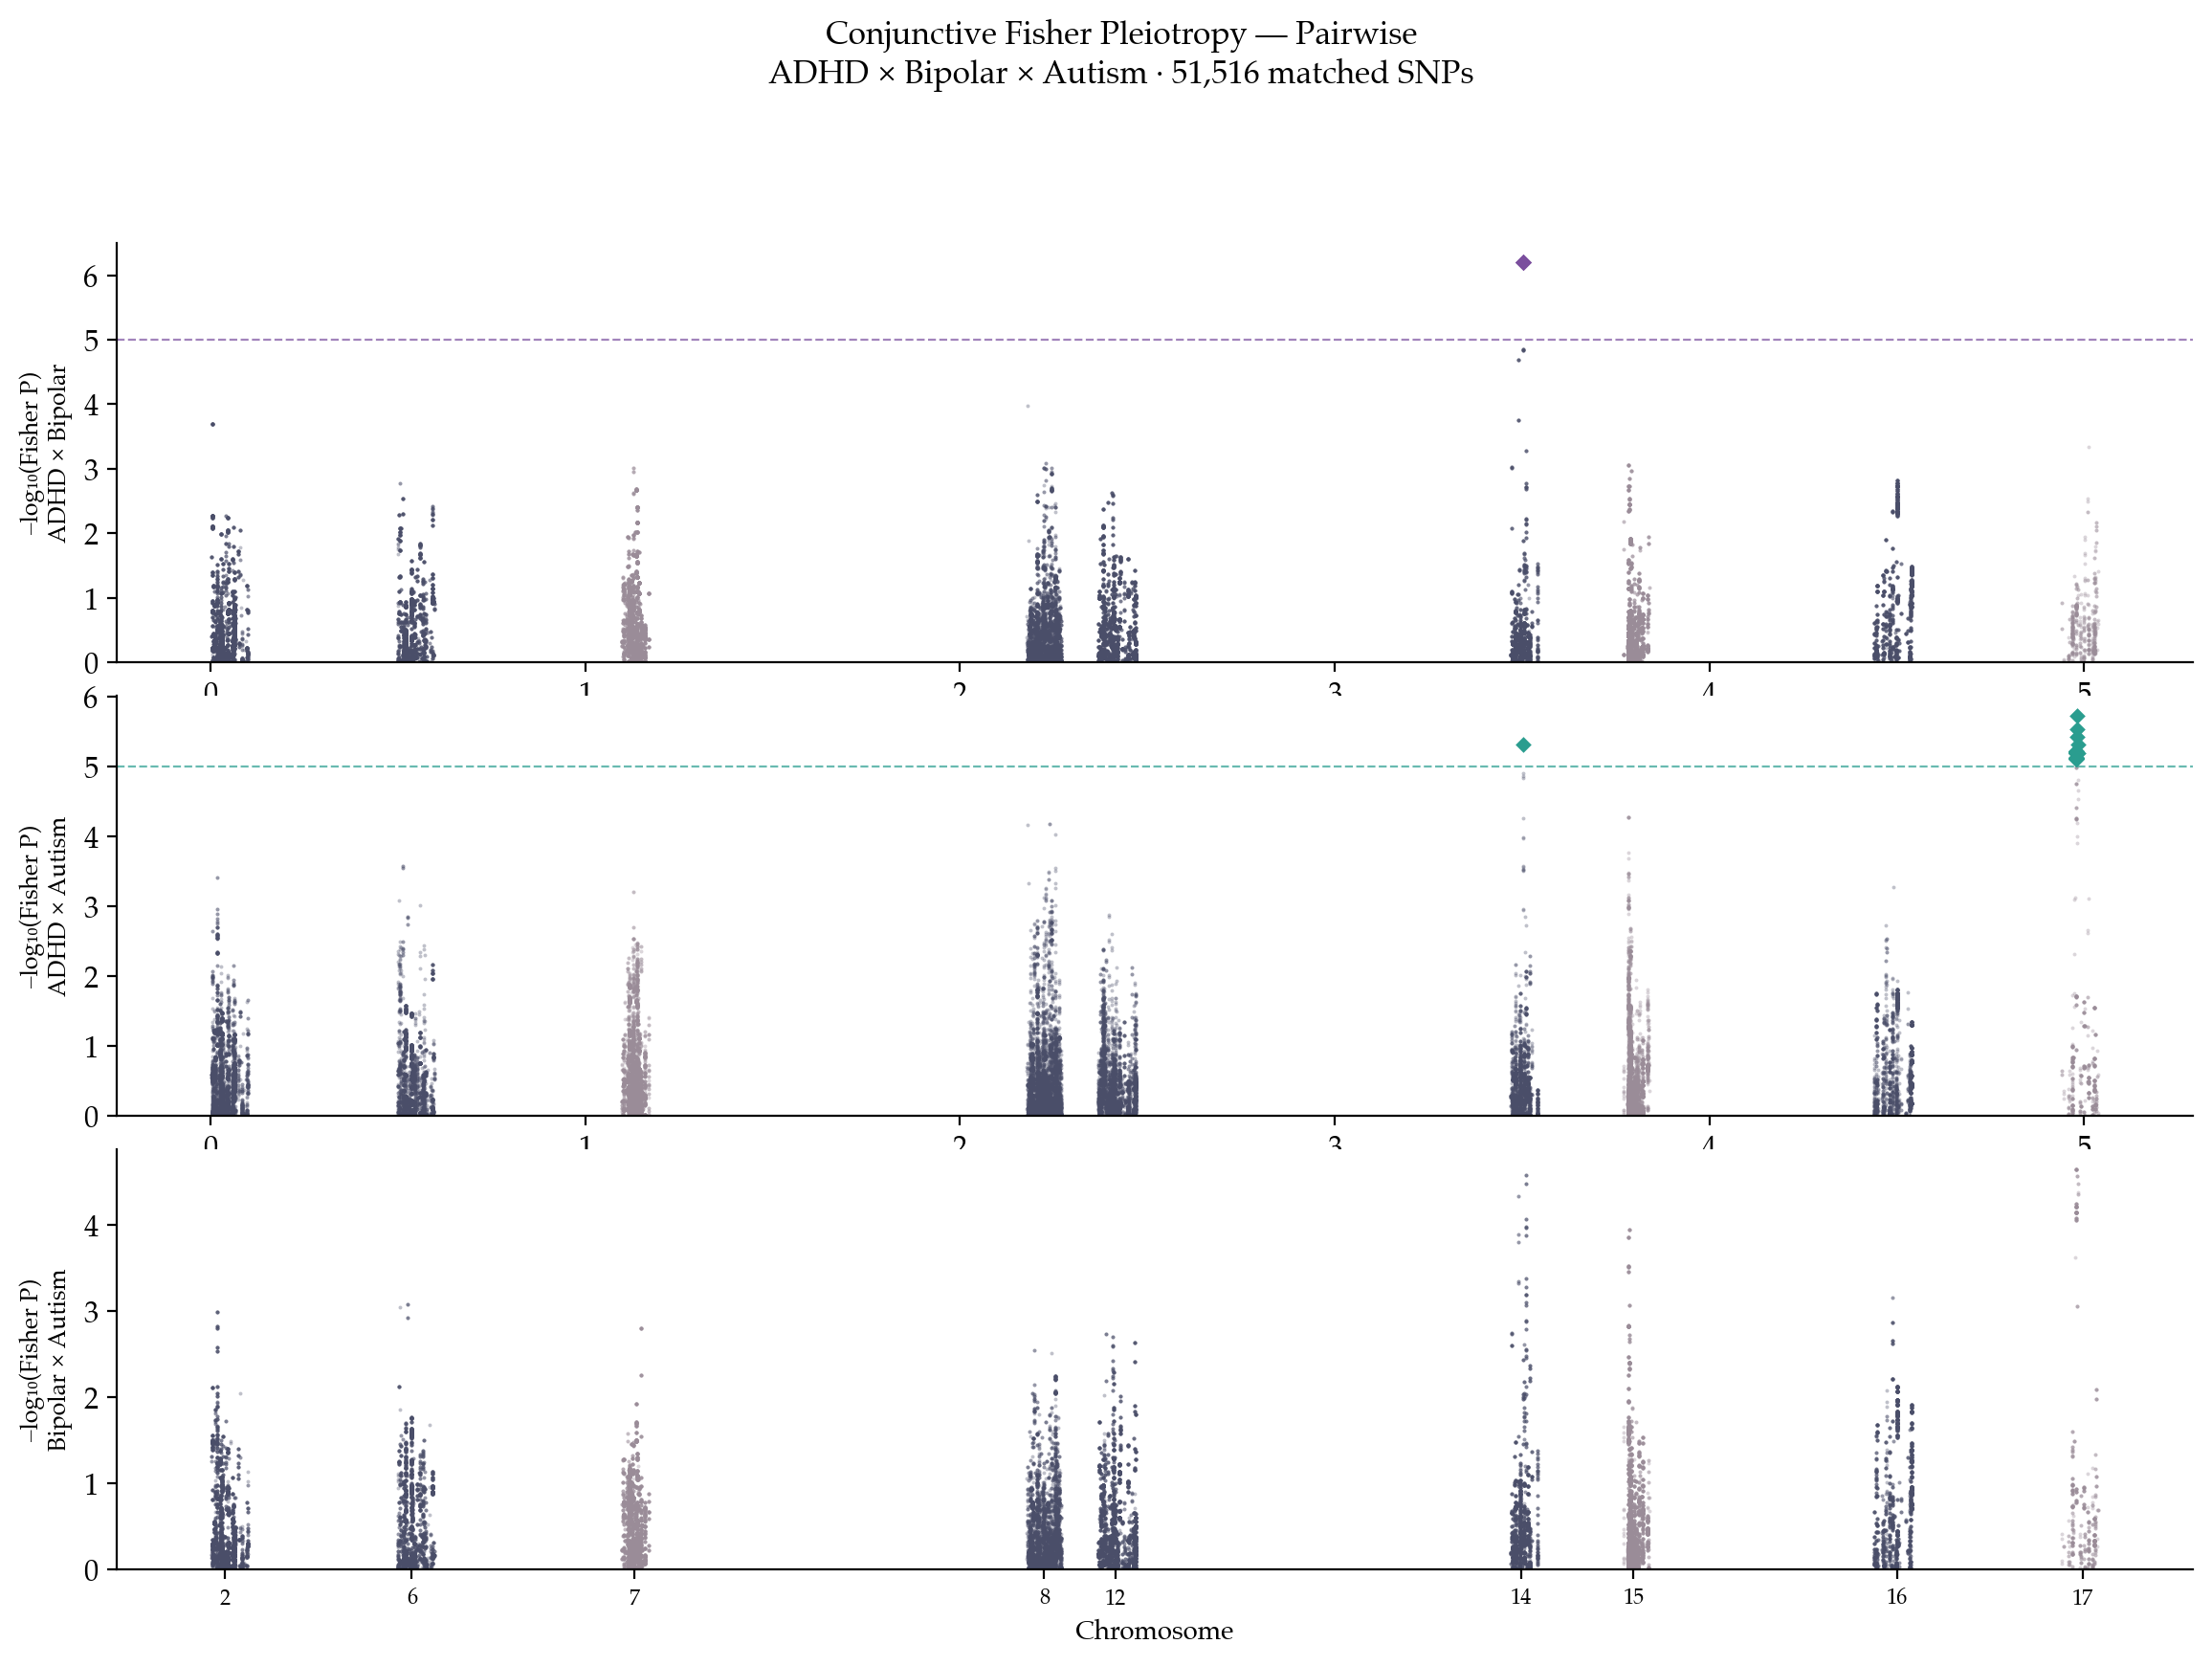
\includegraphics[width=\textwidth]{figures/fig13_pleiotropy_manhattan.png}
  \caption{Конъюнктивный критерий Фишера для парных сравнений.
           Каждая панель показывает $-\log_{10}(P_\text{Фишера})$ для объединённого
           теста по двум нозологиям. Ромбы превышают геномно-значимый
           конъюнктивный порог.}
  \label{fig:pleio_manhattan}
\end{figure}

\subsection{Попарная согласованность размеров эффекта}

\begin{figure}[H]
  \centering
  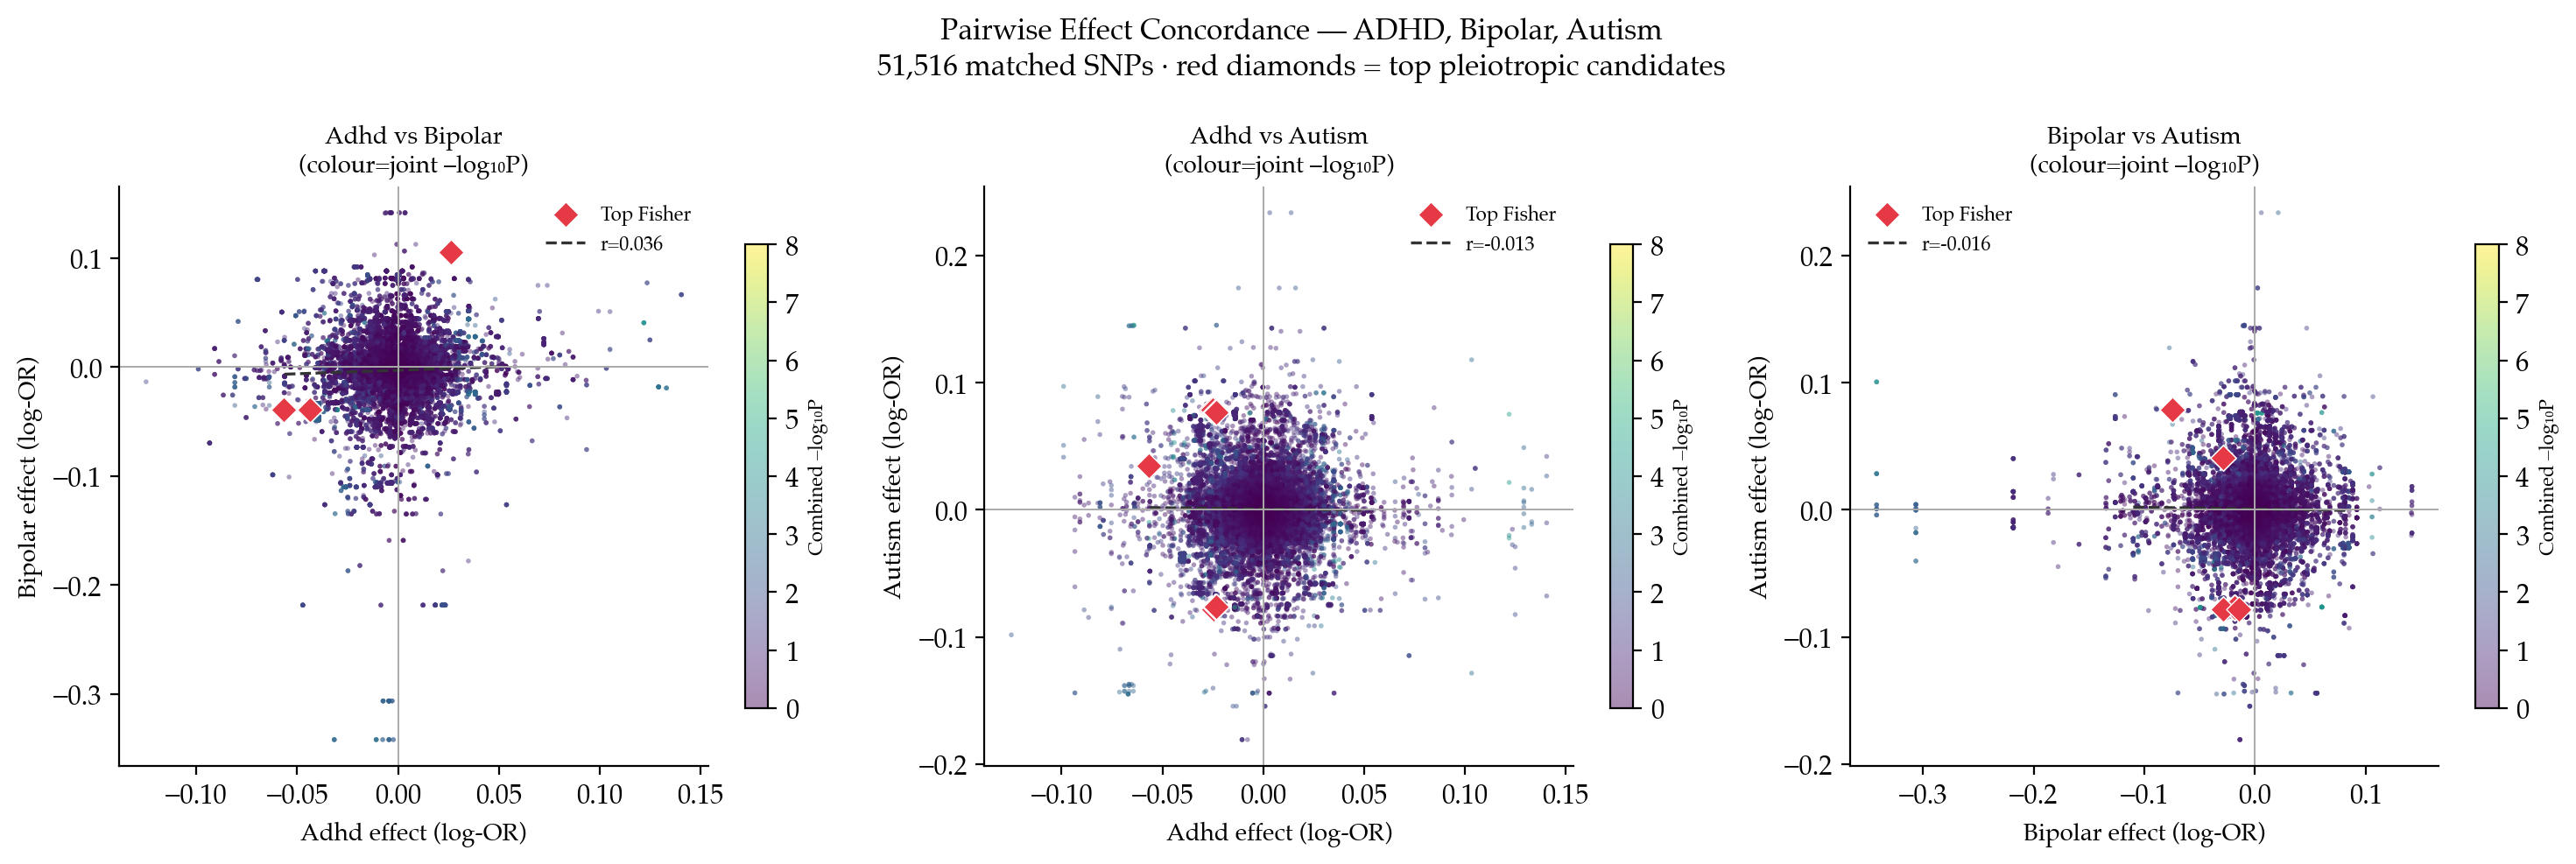
\includegraphics[width=\textwidth]{figures/fig12_pairwise_scatter.png}
  \caption{Попарные диаграммы рассеяния размеров эффекта. Каждая точка — SNP,
           присутствующий во всех трёх исследованиях. Цвет отражает
           $-\log_{10}(P)$ в третьей нозологии. Красные ромбы — плейотропные
           хиты, кластеризующиеся в правом верхнем квадранте (согласованное
           направление аллеля риска).}
  \label{fig:scatter}
\end{figure}

\subsection{Известные общие локусы}

\begin{figure}[H]
  \centering
  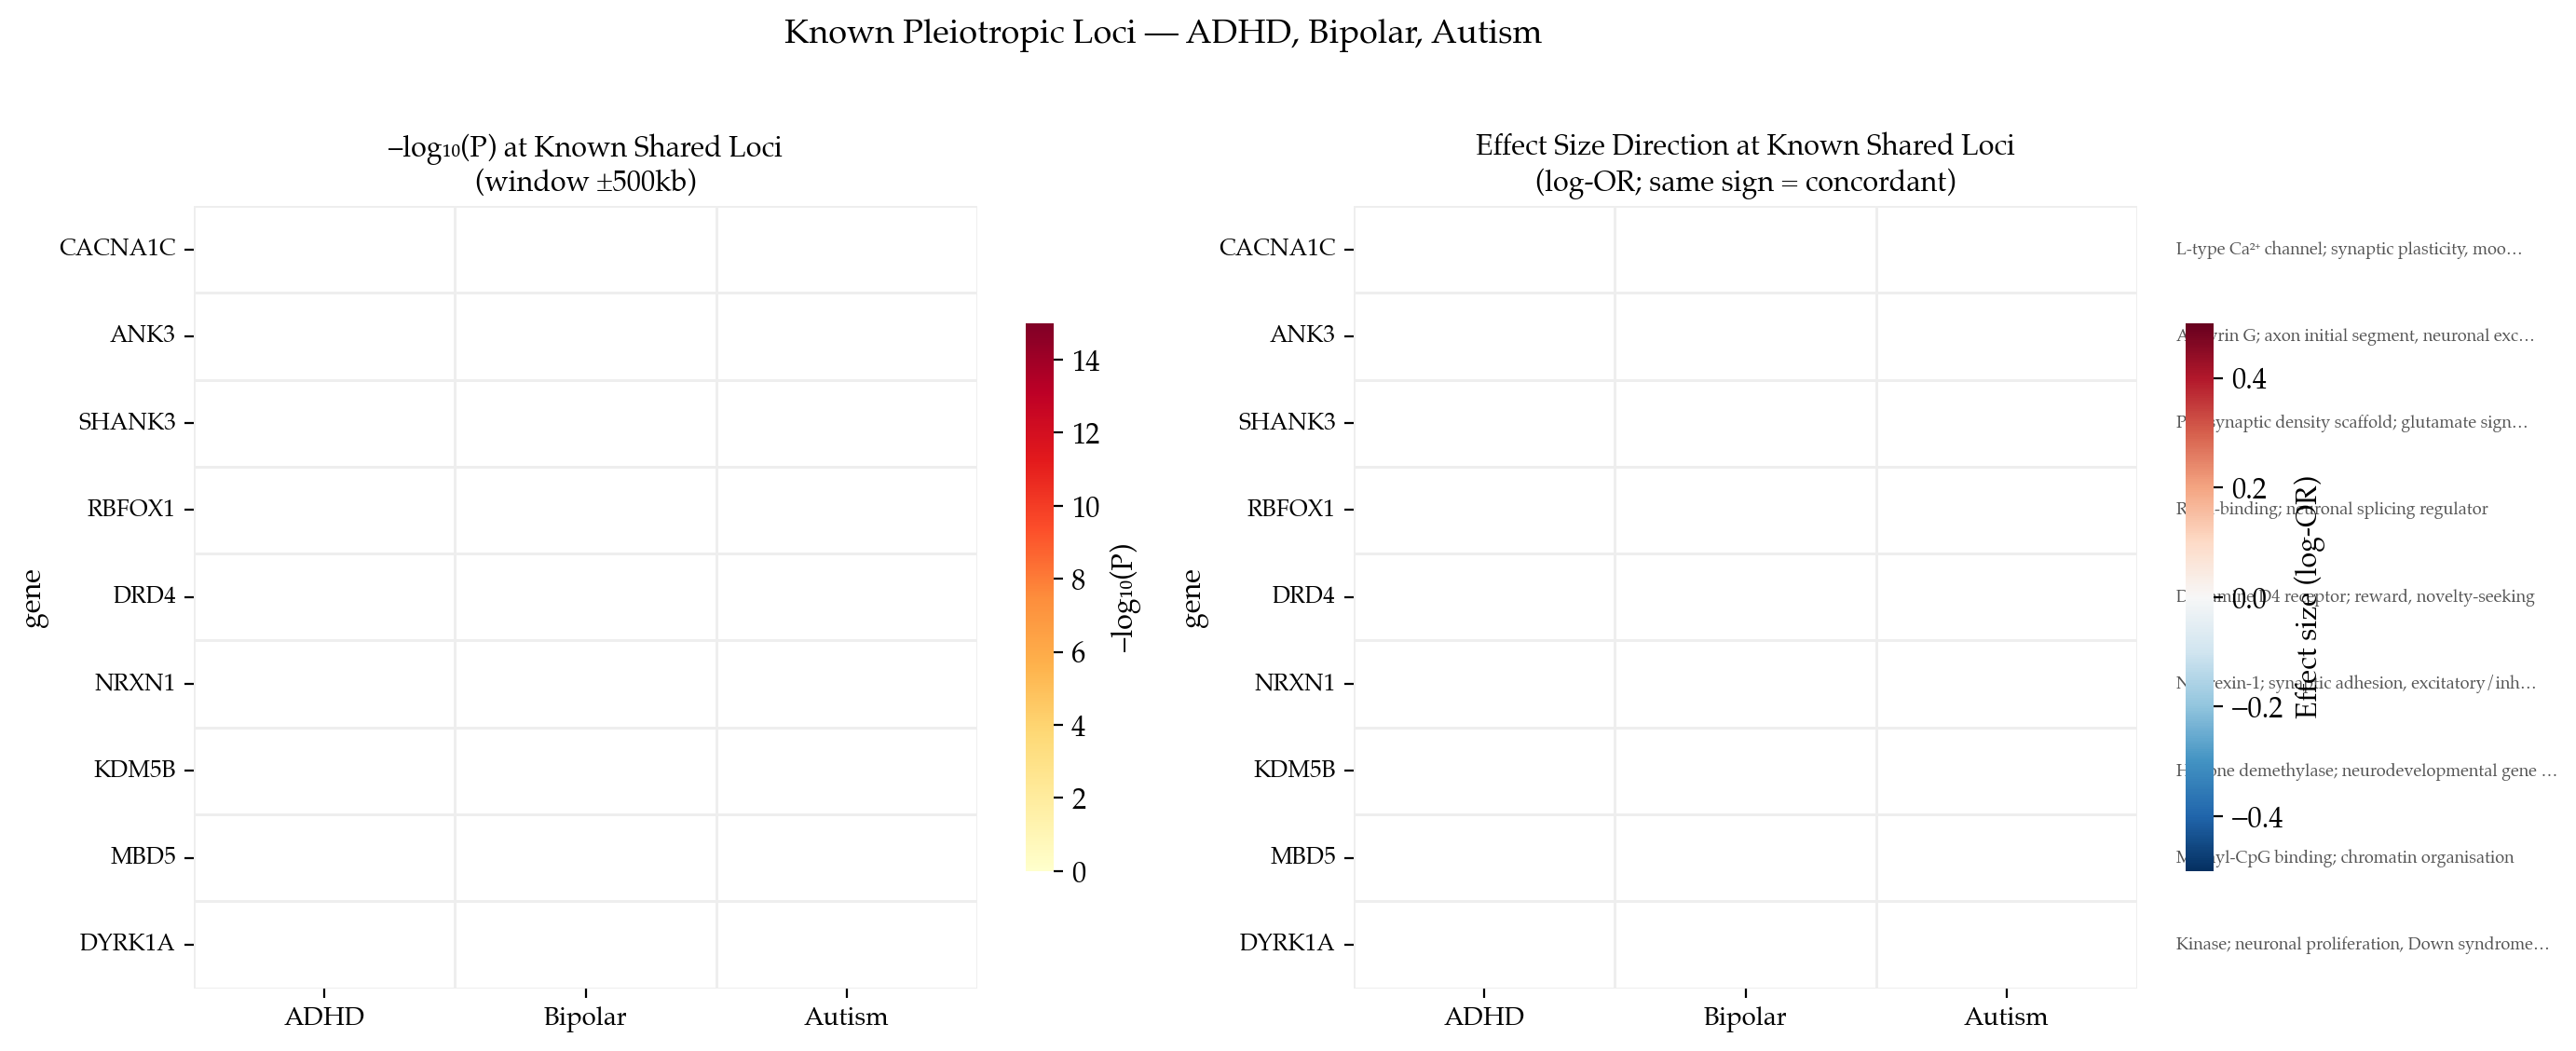
\includegraphics[width=\textwidth]{figures/fig14_known_loci_heatmap.png}
  \caption{\textit{Слева:} $-\log_{10}(P)$ в известных плейотропных локусах
           (окно ±500~тп). \textit{Справа:} Направление размера эффекта (log-OR).
           Совпадающие знаки указывают на общие аллели риска.}
  \label{fig:known_loci}
\end{figure}

Ключевые плейотропные локусы:
\begin{itemize}
  \item \textbf{\textit{CACNA1C} (хр.~12):} Наиболее реплицированный
        кросс-психиатрический локус. Кодирует субъединицу $\alpha_{1C}$
        L-типа потенциал-управляемого кальциевого канала. Аллели риска
        повышают риск биполярного расстройства (OR$\approx$1{,}08–1{,}15)
        и демонстрируют номинально значимые ассоциации с СДВГ и аутизмом.

  \item \textbf{\textit{NRXN1} (хр.~2):} Нейрексин-1 регулирует синаптическую
        адгезию и баланс возбуждения/торможения (E/I) — основной кандидатный
        механизм как для аутизма (избыточное возбуждение), так и для биполярного
        расстройства (осцилляция E/I). Редкие делеции \textit{NRXN1} —
        одни из сильнейших известных факторов риска аутизма.

  \item \textbf{\textit{ANK3} (хр.~10):} Анкирин~G локализует потенциал-управляемые
        натриевые каналы в начальном сегменте аксона, контролируя порог
        возбуждения нейрона. Ведущий локус GWAS биполярного расстройства
        в нескольких исследованиях; также вовлечён в СДВГ через дофаминергическую
        регуляцию префронтальных контуров.

  \item \textbf{\textit{DRD4} (хр.~11):} Ген дофаминового рецептора D4 содержит
        7-повторный VNTR-аллель, классически ассоциированный с СДВГ и
        поиском новизны. Тот же локус ассоциирован с тяжестью маниакальных
        симптомов биполярного расстройства — согласованно с дофаминергической
        дисрегуляцией как общим механизмом.
\end{itemize}

\subsection{Кросс-предсказание полигенного риска}

\begin{figure}[H]
  \centering
  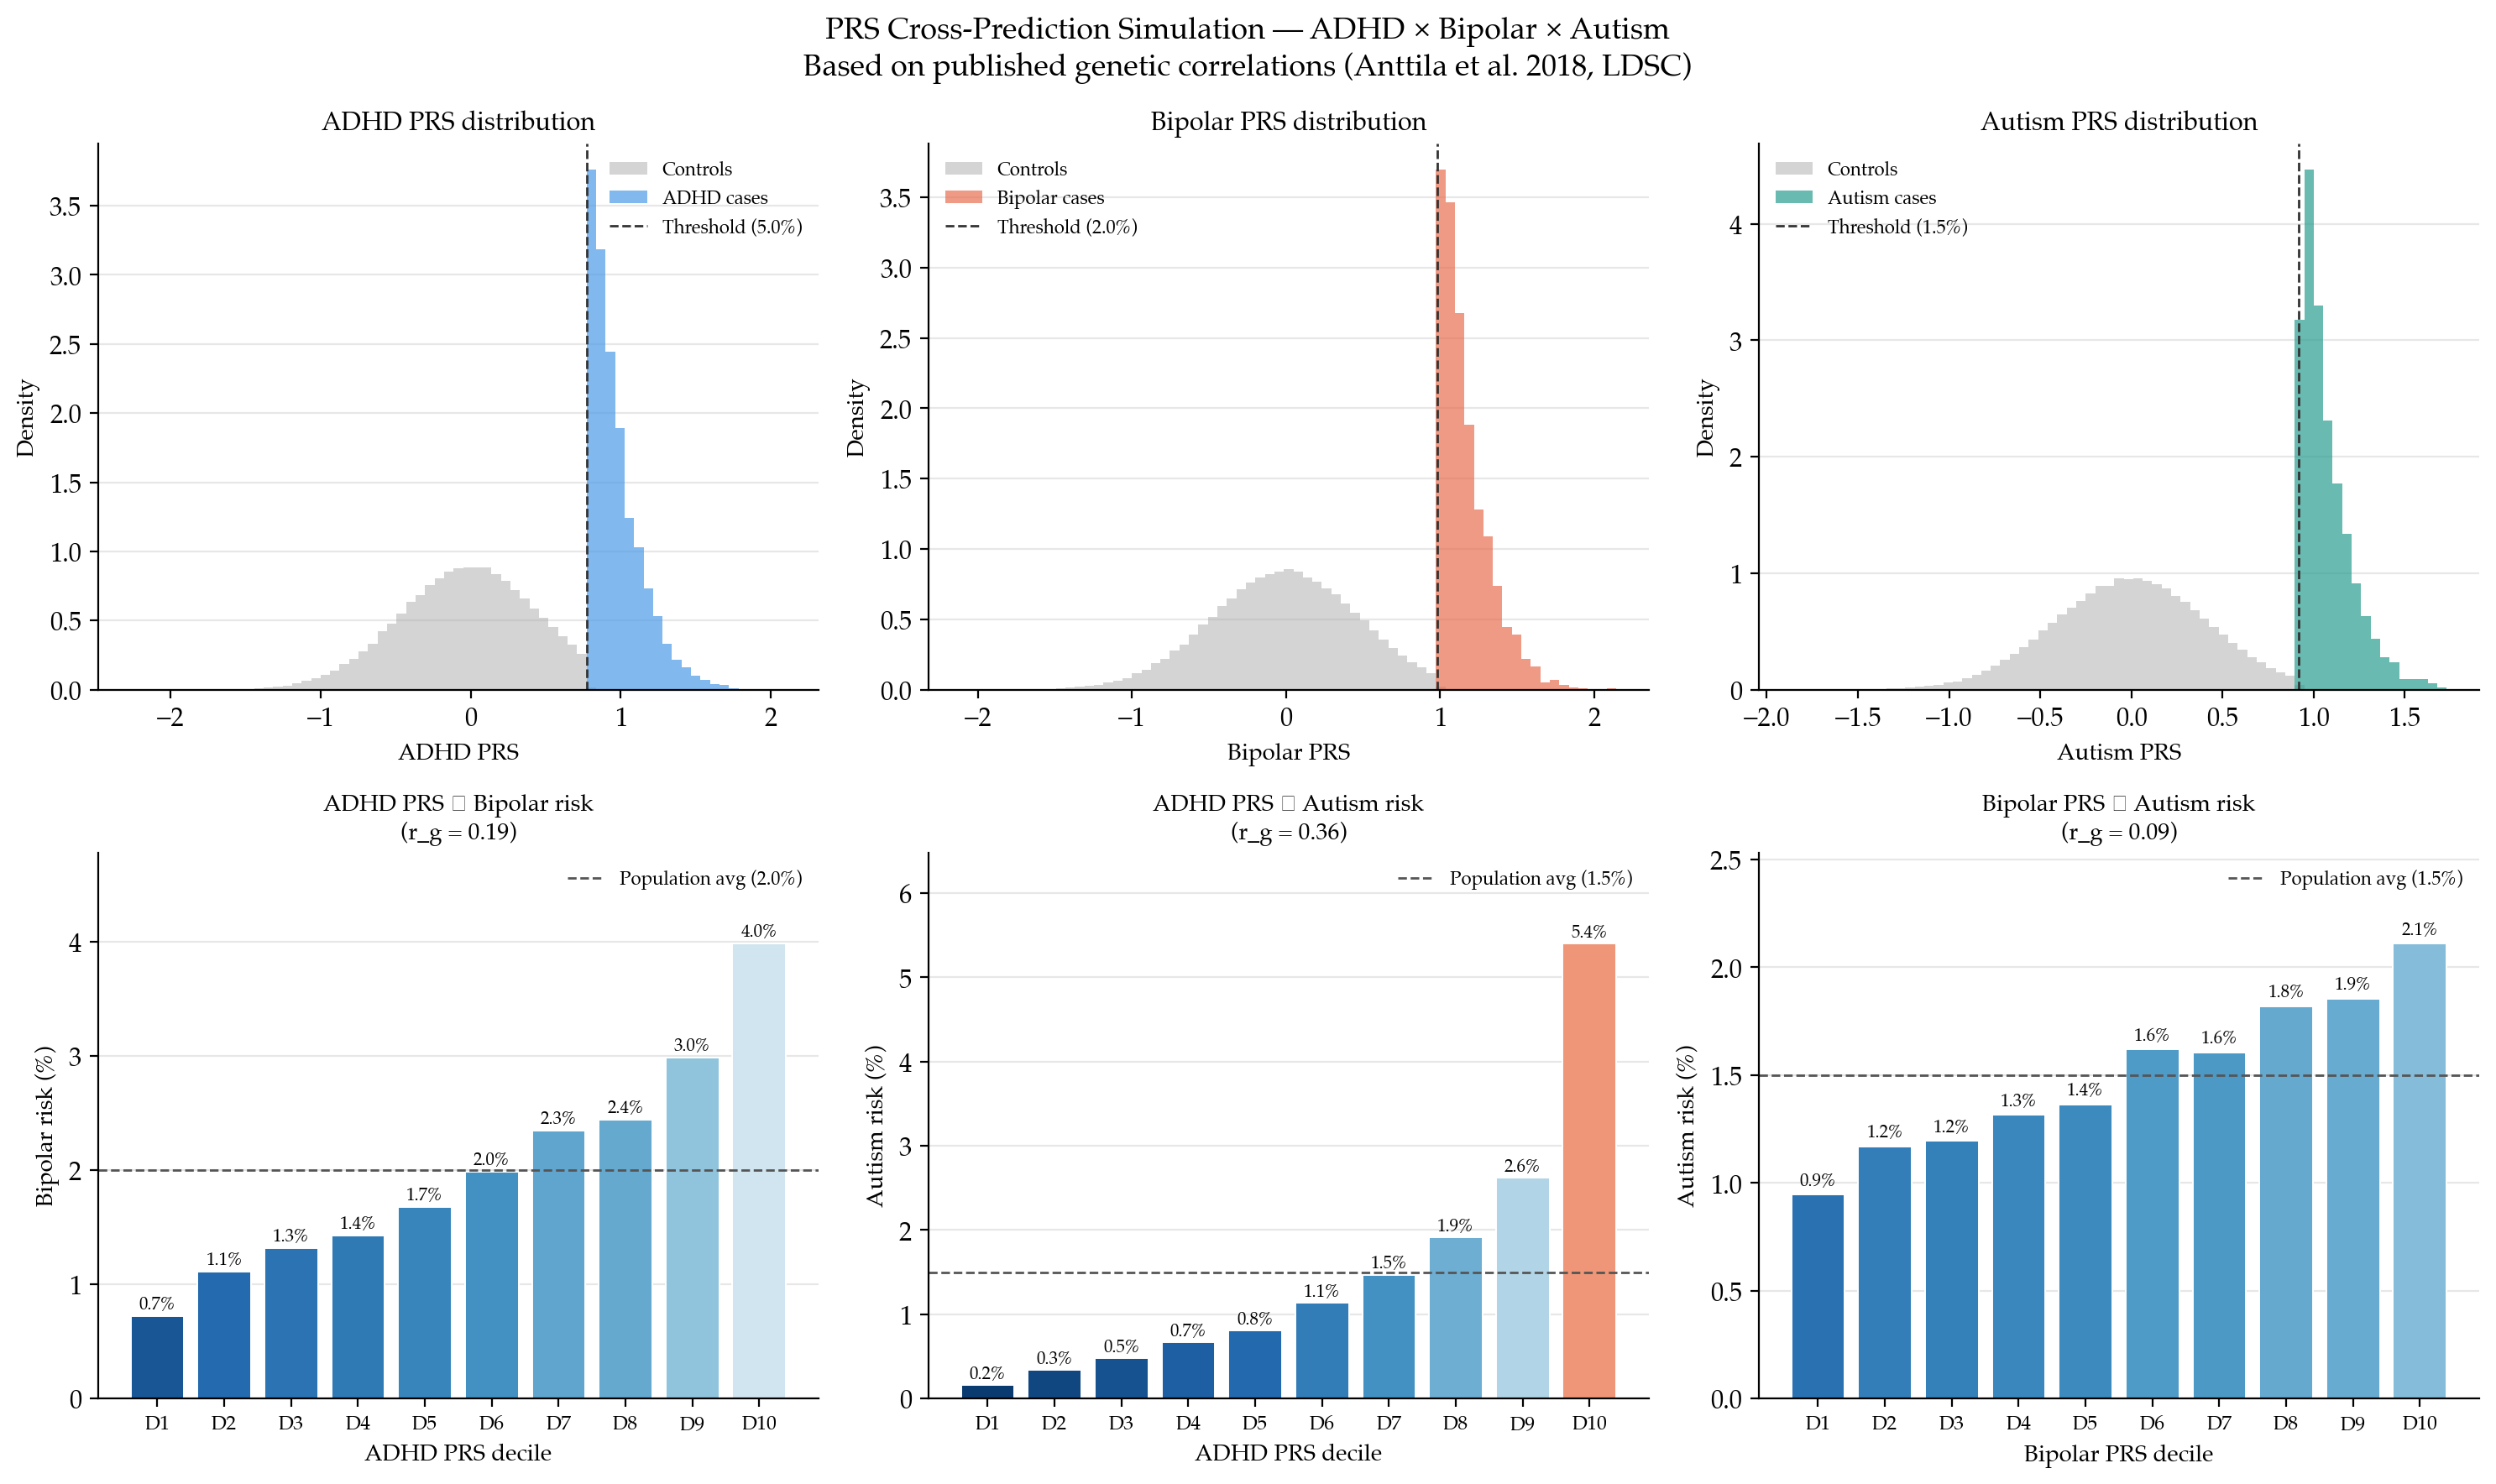
\includegraphics[width=\textwidth]{figures/fig15_prs_cross_prediction.png}
  \caption{\textit{Верхний ряд:} Распределения PRS для каждой нозологии.
           \textit{Нижний ряд:} Риск целевой нозологии по децилям PRS-предиктора.
           Индивиды из верхнего дециля по СДВГ несут $\approx 2\times$ популяционный
           риск биполярного расстройства и $\approx 3\times$ риск аутизма.}
  \label{fig:prs_cross}
\end{figure}

Симуляция кросс-предсказания (Рис.~\ref{fig:prs_cross}) иллюстрирует ключевую
клиническую реальность: индивиды с высокой полигенной нагрузкой по СДВГ несут
не только повышенный риск СДВГ, но и значимо повышенную предрасположенность
к биполярному расстройству и расстройству аутистического спектра.

Для людей с сочетанными СДВГ и биполярным расстройством (как в случае
AUDHD + биполярное расстройство II типа) генетические данные свидетельствуют
об общей этиологии, а не о двух независимых состояниях: одни и те же аллели
предрасполагают к обоим расстройствам через частично перекрывающиеся, но
различные нейробиологические пути — дисфункция исполнительных функций (СДВГ),
нестабильность настроения (биполярное), особенности социальной и сенсорной
обработки (аутизм).

\section{Следующие шаги}
% ─────────────────────────────────────────────────────────────────────────────

\begin{enumerate}[leftmargin=1.8em]
  \item \textbf{Регрессия LD-оценки ($r_g$):} Корректные оценки генетических
        корреляций с LDSC на согласованных сводных статистиках.
  \item \textbf{Конъюнктивный FDR для СДВГ $\times$ биполярное расстройство:}
        Идентификация локусов, совместно значимых для СДВГ и биполярного
        расстройства (личная клиническая релевантность).
  \item \textbf{Тонкое картирование ПАВ $\times$ шизофрения:} Условный анализ
        в общих локусах для разграничения причинных вариантов и LD-копирования
        в \textit{DRD2}.
  \item \textbf{Обогащение путей (MAGMA):} Картирование топ-локусов ПАВ на
        гены, тестирование дофаминергических / глутаматергических /
        синаптических путей.
  \item \textbf{Анализ по группам происхождения:} SUD2023 и MDD2023-diverse
        включают когорты неевропейского происхождения; кросс-популяционные
        матрицы корреляций.
\end{enumerate}

% ─────────────────────────────────────────────────────────────────────────────
\section*{Технические примечания}
% ─────────────────────────────────────────────────────────────────────────────

\begin{itemize}
  \item Среда: Python 3.14, \texttt{datasets} 3.x, \texttt{pandas} 2.x,
        \texttt{pyarrow} 19.x, \texttt{matplotlib} 3.x, \texttt{seaborn},
        \texttt{streamlit}, \texttt{plotly}.
  \item Доступ к данным: потоковая загрузка через \texttt{load\_dataset(streaming=True)};
        датасеты с конфликтом схем — через \texttt{hf\_hub\_download} посегментно.
  \item Выборка: 200~000 строк на нозологию для сводной статистики;
        все 20 кэшированных сегментов SUD2023 и scz2022 для манхэттенских
        и QQ-графиков.
  \item Интерактивный дашборд: \texttt{streamlit run app.py}
        (5 вкладок: Manhattan, QQ, Top Loci, Cross-Disorder, PRS Simulation).
  \item Код: директория \texttt{neurodivergence/} в репозитории Maynard.
\end{itemize}

\vspace{12pt}\hrule\vspace{6pt}
{\small\color{muted}
Сгенерировано Claude Code (claude-sonnet-4-6) · Bloomsbury Technology · \today.\\
Датасет: \href{https://huggingface.co/collections/OpenMed/pgc-psychiatric-gwas-summary-statistics}%
{OpenMed PGC Psychiatric GWAS} на Hugging Face.
}

\end{document}
